\documentclass[12pt, twoside]{book}
\input{latex-settings.tex}

% STRONA TYTULOWA - title_page/pd_mgr_pl.pdf
\frontmatter
\begin{document}

\includepdf[pages={1}]{title_page/pd_mgr_pl.pdf}
\doublepage

% STRESZCZENIA (PL + ANG) - chapters/abstract.tex
\pagestyle{tableOfContentStyle}
\pagenumbering{Roman}
\section*{Streszczenie}

Zmiana modelu licencjonowania Redis po wersji~7.2 postawiła organizacje korzystające z~tego systemu cache'ującego przed decyzją o~dalszej ścieżce rozwoju infrastruktury. Niniejsza praca przedstawia kompleksową analizę porównawczą trzech rozwiązań: samodzielnie zarządzanego klastra Valkey w~Kubernetes, klastra Redis~7.2 oraz usługi zarządzanej Google Cloud Memorystore for Redis. Celem było ustalenie, czy Valkey stanowi praktyczną, wydajną i~ekonomicznie uzasadnioną alternatywę dla Redis~7.2 i~rozwiązania zarządzanego.

Przeprowadzono siedem kategorii testów --- badania wydajności, resharding, failover mastera, spójność danych podczas partycji sieciowej, odporność na niedobór zasobów CPU i~pamięci, rolling upgrade oraz backup i~restore --- każdy powtarzany pięciokrotnie. Wyniki poddano analizie statystycznej z~wykorzystaniem testu Manna-Whitneya~U oraz korekty Benjaminiego-Hochberga przy porównaniach wielokrotnych.

Wykazano, że Valkey osiąga istotnie wyższą przepustowość niż Redis~7.2 w~większości profili obciążenia przy nieodróżnialnym statystycznie zachowaniu podczas failoveru i~partycji sieciowej. Infrastruktura self-hosted okazała się tańsza od usługi zarządzanej, kosztem wyższego nakładu pracy operacyjnej. Wyniki potwierdzają, że Valkey jest dojrzałym zamiennikiem Redis~7.2 w~środowiskach chmurowych.

\section*{Abstract}

The change in the Redis licensing model after version~7.2 confronted organizations relying on this caching system with a~decision about the future direction of their infrastructure. This thesis presents a~comprehensive comparative analysis of three solutions: a~self-managed Valkey cluster on Kubernetes, a~Redis~7.2 cluster, and the managed Google Cloud Memorystore for Redis service. The goal was to determine whether Valkey constitutes a~practical, performant, and economically justified alternative to Redis~7.2 and to the managed offering.

Seven categories of tests were conducted --- baseline performance, resharding, master failover, data consistency during a~network partition, resilience to CPU and memory pressure, rolling upgrade, and backup and restore --- each repeated five times. The results were analysed statistically using the Mann-Whitney~U test with the Benjamini-Hochberg correction for multiple comparisons.

The study shows that Valkey achieves significantly higher throughput than Redis~7.2 across most workload profiles, while behaving in a~statistically indistinguishable manner during failover and network partitions. The self-hosted infrastructure proved cheaper than the managed service, at the cost of higher operational effort. The results confirm that Valkey is a~mature drop-in replacement for Redis~7.2 in cloud environments.

\doublepage

% SPIS TRESCI
\tableofcontents
\doublepage

% ROZDZIALY - chapters/*.tex
\pagestyle{custom}
\mainmatter
\chapter{Wstęp}\label{ch:wstep}

Systemy cache'owania danych w pamięci operacyjnej są jednym z podstawowych elementów współczesnych architektur aplikacji internetowych i chmurowych. Ich zadaniem jest ograniczenie liczby kosztownych odwołań do baz danych, usług zewnętrznych lub warstw trwałego składowania poprzez utrzymywanie często wykorzystywanych danych w strukturach dostępnych z bardzo małym opóźnieniem. W praktyce rozwiązania tego typu wpływają bezpośrednio na czas odpowiedzi aplikacji, stabilność systemu podczas skoków obciążenia oraz koszty działania infrastruktury. Znaczenie Redis jako narzędzia cache'ującego w aplikacjach o dużym ruchu zostało opisane między innymi w pracy Kaptosva, w której wskazano, że właściwie zaprojektowana warstwa cache może istotnie ograniczać opóźnienia i odciążać komponenty odpowiedzialne za trwałe przechowywanie danych~\cite{kaptosv2025}.

Redis przez wiele lat był jednym z najczęściej wybieranych rozwiązań typu in-memory data store. Jego popularność wynikała z prostego modelu danych, wysokiej wydajności, szerokiego wsparcia narzędziowego oraz dojrzałego ekosystemu bibliotek klienckich. Jednocześnie zmiany licencyjne wprowadzone po wersji Redis 7.2 spowodowały istotną zmianę w sposobie postrzegania tego projektu przez społeczność open-source oraz dostawców usług chmurowych. Problem wpływu zmiany licencji Redis na ekosystem oprogramowania otwartego i dostawców usług chmurowych został omówiony przez Hana i współautorów~\cite{han2026}. Jedną z odpowiedzi społeczności na te zmiany było powstanie projektu Valkey, rozwijanego jako otwarta alternatywa zgodna funkcjonalnie z wcześniejszym kierunkiem rozwoju Redis. Awaysheh i Awad wskazują Valkey jako jeden z przykładów nowej generacji chmurowo-natywnych magazynów danych w pamięci, obok innych systemów rozwijanych w odpowiedzi na wymagania nowoczesnych środowisk obliczeniowych~\cite{awaysheh2025}.

Z punktu widzenia organizacji wykorzystujących cache w środowiskach produkcyjnych sama zgodność interfejsu nie jest jednak wystarczającą podstawą do podjęcia decyzji o migracji. Wybór między Redis, Valkey oraz usługami zarządzanymi wymaga oceny wielu aspektów jednocześnie: wydajności, opóźnień, odporności na awarie, kosztów infrastruktury oraz nakładu pracy administracyjnej. Szczególnie istotne jest to w środowiskach Kubernetes, w których zespoły mogą samodzielnie utrzymywać klastry bazujące na kontenerach, operatorach i mechanizmach automatycznego odtwarzania. Takie podejście może obniżać koszty i zwiększać kontrolę nad konfiguracją, ale jednocześnie przenosi na zespół odpowiedzialność za aktualizacje, monitoring, kopie zapasowe, skalowanie oraz reakcję na awarie.

\section{Przedmiot pracy}

Przedmiotem pracy jest analiza porównawcza klastra Valkey uruchomionego w środowisku Kubernetes z rozwiązaniami opartymi o Redis. Badanie koncentruje się na scenariuszach typowych dla warstwy cache w aplikacjach chmurowych, w których kluczowe znaczenie mają duża liczba operacji na sekundę, niskie opóźnienia oraz przewidywalne zachowanie systemu pod obciążeniem. W pracy rozpatrywane są zarówno testy wydajnościowe, jak i wybrane aspekty utrzymywalności oraz niezawodności, ponieważ w praktyce produkcyjnej wysoka przepustowość nie jest wystarczająca, jeśli system jest trudny w aktualizacji, niestabilny podczas awarii lub kosztowny w obsłudze.

Problem badawczy można sformułować następująco: czy samodzielnie zarządzany klaster Valkey w Kubernetes może stanowić praktyczną, wydajną i ekonomicznie uzasadnioną alternatywę dla klastra Redis oraz usług zarządzanych, przy zachowaniu akceptowalnego poziomu niezawodności i złożoności operacyjnej? Odpowiedź na to pytanie wymaga nie tylko porównania wartości średnich dla liczby operacji na sekundę, ale również analizy rozkładu opóźnień, zachowania przy różnych rozmiarach danych, wpływu liczby przydzielonych zasobów CPU oraz skutków awarii lub operacji administracyjnych wykonywanych podczas ciągłego obciążenia.

Istotnym elementem przedmiotu badań jest środowisko uruchomieniowe. Testy zakładają pracę w Kubernetes, ponieważ jest to obecnie jeden z podstawowych sposobów wdrażania usług stanowych i bezstanowych w środowiskach chmurowych. W takim modelu sam mechanizm działania bazy in-memory nie jest jedynym czynnikiem wpływającym na wynik. Znaczenie mają również limity zasobów, sposób rozmieszczenia podów, narzut sieciowy wewnątrz klastra, mechanizmy odtwarzania replik oraz integracja z monitoringiem. Z tego powodu praca nie ogranicza się do syntetycznego uruchomienia pojedynczego procesu Redis lub Valkey, lecz traktuje badany system jako usługę działającą w rzeczywistym modelu wdrożeniowym.

\section{Cele pracy}

Celem głównym pracy jest przeprowadzenie kompleksowej analizy porównawczej samodzielnie zarządzanego klastra Valkey uruchomionego w Kubernetes z rozwiązaniami opartymi o Redis, z uwzględnieniem wydajności, opóźnień, odporności na awarie, kosztów oraz nakładu pracy operacyjnej. Wyniki badań mają umożliwić ocenę, w jakich warunkach Valkey może być traktowany jako technicznie i ekonomicznie uzasadniona alternatywa dla Redis Cluster lub usługi zarządzanej.

Cel główny został rozbity na następujące cele szczegółowe:

\begin{itemize}
    \item przygotowanie środowiska testowego w Kubernetes dla badanych wariantów systemu cache;
    \item opracowanie powtarzalnej procedury testów wydajnościowych z wykorzystaniem narzędzia \texttt{memtier\_benchmark};
    \item porównanie przepustowości oraz opóźnień dla różnych konfiguracji CPU, rozmiarów danych i proporcji operacji odczytu oraz zapisu;
    \item zbadanie zachowania klastra podczas awarii, niedoboru zasobów, aktualizacji oraz wybranych operacji administracyjnych;
    \item określenie kosztów oraz nakładu pracy operacyjnej dla wariantu self-hosted w porównaniu z rozwiązaniem zarządzanym;
    \item sformułowanie rekomendacji dotyczących wykorzystania Valkey i Redis w środowiskach chmurowych.
\end{itemize}

W pracy przyjęto cztery hipotezy badawcze:

\begin{itemize}
    \item \textbf{H1:} klaster Valkey osiąga większą przepustowość oraz niższe opóźnienia p95, p99 i p99.9 niż Redis Cluster przy takim samym przydziale zasobów CPU;
    \item \textbf{H2:} samodzielnie zarządzany klaster Valkey może być tańszy od usługi zarządzanej przy porównywalnej wydajności i dostępności;
    \item \textbf{H3:} czas odtworzenia mastera po awarii w rozwiązaniach zintegrowanych z Kubernetes jest krótszy niż w klasycznym podejściu Redis Sentinel oraz porównywalny z mechanizmami usług zarządzanych;
    \item \textbf{H4:} samodzielnie utrzymywany klaster Valkey wymaga większego nakładu pracy operacyjnej niż usługa zarządzana, mimo potencjalnych korzyści wydajnościowych i kosztowych.
\end{itemize}

\section{Zakres i ograniczenia pracy}

Zakres pracy obejmuje testy wydajnościowe, testy odpornościowe oraz analizę utrzymywalności. W części wydajnościowej badane są operacje odczytu, zapisu oraz mieszane scenariusze odczytu i zapisu. Zmiennymi niezależnymi są liczba vCPU przypisana do poda, rozmiar payloadu oraz proporcja typów operacji. Dla każdej konfiguracji wykonywana jest seria powtórzeń, a wyniki są analizowane z wykorzystaniem średniej, odchylenia standardowego oraz percentyli opóźnień. Takie podejście jest spójne z charakterem badań systemów in-memory, w których pojedyncza wartość średnia może ukrywać istotne problemy widoczne dopiero w ogonie rozkładu opóźnień.

W części dotyczącej niezawodności i utrzymywalności uwzględniono scenariusze failover, presję na zasoby CPU i pamięć, aktualizację klastra podczas obciążenia, skalowanie horyzontalne oraz operacje backupu i odtwarzania. Scenariusze te zostały dobrane tak, aby odzwierciedlały zadania, z którymi administratorzy i zespoły platformowe spotykają się w środowiskach produkcyjnych. Analiza nie ogranicza się więc wyłącznie do parametrów szybkościowych, ale obejmuje również praktyczną ocenę trudności utrzymania badanego rozwiązania.

Praca ma również ograniczenia. Testy wykonywane są w kontrolowanym środowisku laboratoryjnym, dlatego ich wyniki nie muszą wprost odpowiadać wszystkim możliwym konfiguracjom produkcyjnym. Na rezultaty mogą wpływać parametry klastra Kubernetes, zasoby komputera testowego, konfiguracja sieci, wersje obrazów kontenerowych oraz sposób działania narzędzia generującego obciążenie. Ponadto porównanie z usługą zarządzaną ma częściowo charakter black-box, ponieważ dostawcy chmurowi nie zawsze ujawniają szczegóły wewnętrznej implementacji mechanizmów failover, replikacji i backupu. Ograniczenia te są jednak typowe dla badań porównawczych systemów infrastrukturalnych i zostaną uwzględnione podczas interpretacji wyników.

\section{Struktura pracy}

Praca składa się z sześciu rozdziałów merytorycznych. Rozdział~\ref{ch:wstep} przedstawia kontekst problemu, przedmiot badań, cele pracy, hipotezy oraz zakres i ograniczenia opracowania. Rozdział~\ref{ch:tematyka} zawiera teoretyczne podstawy problematyki badań, w tym omówienie systemów cache'owania, architektury Redis i Valkey, modeli klastrowych oraz znaczenia zmian licencyjnych dla ekosystemu open-source. Rozdział~\ref{ch:organizacja} opisuje założenia metodologiczne, środowisko badawcze, wykorzystywane narzędzia, konfiguracje testowe oraz plan eksperymentów.

W rozdziale~\ref{ch:wyniki} przedstawione zostaną wyniki pomiarów wydajnościowych, testów odpornościowych i analiz operacyjnych. Rozdział~\ref{ch:podsumowanie} będzie poświęcony syntetycznemu omówieniu rezultatów, weryfikacji hipotez badawczych oraz sformułowaniu wniosków wynikających z przeprowadzonych badań. Rozdział~\ref{ch:zakonczenie} zamknie pracę poprzez wskazanie najważniejszych osiągnięć, ograniczeń oraz możliwych kierunków dalszych badań.

\chapter{Teoretyczne podstawy problematyki badań}\label{ch:tematyka}

Poniżej przedstawiono pojęcia i technologie stanowiące fundament dalszych rozdziałów: systemy cache, architekturę Redis i Valkey, kontekst licencyjny, środowisko Kubernetes oraz różnice między modelami zarządzanymi a self-hosted.

\section{Systemy cache'owania w pamięci operacyjnej}

Jak wskazano we wstępie, warstwa cache w pamięci operacyjnej wpływa bezpośrednio na czas odpowiedzi aplikacji, stabilność systemu podczas skoków obciążenia oraz koszty infrastruktury~\cite{kaptosv2025}. Poniżej omówiono strategie integracji cache z aplikacją, wymagania wobec takich systemów oraz metryki stosowane do ich oceny.

\subsection{Strategie cache'owania}

W literaturze wyróżnia się kilka podstawowych strategii integracji cache z aplikacją~\cite{azureCacheAside, zakhary2017caching}:

\begin{itemize}
    \item \textbf{Cache-aside} (lazy loading) -- aplikacja najpierw sprawdza cache, a w przypadku braku danych (cache miss) pobiera je ze źródła trwałego i zapisuje w cache. Jest to najprostsza i najczęściej stosowana strategia, ponieważ nie wymaga dodatkowej infrastruktury między aplikacją a bazą danych.
    \item \textbf{Read-through} -- cache sam pobiera dane ze źródła w przypadku braku klucza. Z perspektywy aplikacji cache zachowuje się jak jedyne źródło danych.
    \item \textbf{Write-through} -- każdy zapis trafia jednocześnie do cache i do trwałego źródła. Strategia ta zapewnia spójność, ale zwiększa opóźnienie operacji zapisu.
    \item \textbf{Write-behind} (write-back) -- zapis trafia najpierw do cache, a następnie jest asynchronicznie propagowany do źródła trwałego. Zmniejsza opóźnienie zapisu kosztem ryzyka utraty danych w przypadku awarii cache przed propagacją.
\end{itemize}

W systemach produkcyjnych najczęściej stosuje się strategię cache-aside w połączeniu z polityką wygasania kluczy (TTL), ponieważ łączy ona prostotę implementacji z akceptowalnym poziomem spójności danych.

\subsection{Wymagania wobec systemów cache}

Systemy cache wykorzystywane w środowiskach produkcyjnych muszą spełniać jednocześnie kilka wymagań. Podstawowym jest niska latencja odczytu i zapisu, ponieważ celem istnienia warstwy cache jest właśnie skrócenie czasu odpowiedzi. Równie istotna jest wysoka przepustowość, wyrażana jako liczba operacji na sekundę (ops/sec), pozwalająca obsługiwać duży wolumen żądań bez degradacji. Skalowalność horyzontalna umożliwia zwiększanie pojemności i przepustowości przez dodawanie kolejnych węzłów. Opcjonalna trwałość danych pozwala na odtworzenie stanu po restarcie, co jest istotne w scenariuszach, w których ponowne zasilenie cache ze źródła trwałego jest kosztowne czasowo.

\subsection{Metryki oceny systemów cache}

Do oceny wydajności systemów cache stosuje się przede wszystkim liczbę operacji na sekundę (ops/sec) oraz rozkład opóźnień. Wartość średnia opóźnienia jest niewystarczająca, ponieważ może ukrywać problemy widoczne dopiero w ogonie rozkładu. Z tego powodu standardem branżowym jest raportowanie percentyli: p50 (mediana), p95, p99 oraz p99.9. Percentyl p99 oznacza, że 99\% żądań otrzymało odpowiedź w czasie nie dłuższym niż podana wartość, natomiast pozostały 1\% żądań doświadczył wyższych opóźnień. W systemach obsługujących miliony żądań dziennie nawet 0{,}1\% wolnych odpowiedzi może dotyczyć tysięcy użytkowników.

\section{Architektura Redis}

Redis (Remote Dictionary Server) to system bazy danych typu klucz-wartość przechowujący dane w pamięci operacyjnej. Został stworzony przez Salvatore Sanfilippo w 2009 roku i przez ponad dekadę był jednym z najczęściej wybieranych rozwiązań typu in-memory data store~\cite{redisDocumentation}.

\subsection{Model danych}

Redis oferuje bogaty zestaw struktur danych wykraczający poza prosty model klucz-wartość. Podstawowe typy obejmują: ciągi znaków (strings), listy (lists), zbiory (sets), zbiory uporządkowane (sorted sets), tablice mieszające (hashes), bitmapy, strumienie (streams) oraz struktury probabilistyczne (HyperLogLog). Każda z tych struktur udostępnia dedykowane operacje wykonywane atomowo po stronie serwera, co eliminuje konieczność pobierania danych, modyfikowania ich po stronie klienta i odsyłania z powrotem.

\subsection{Model przetwarzania żądań}

Redis wykorzystuje jednowątkowy model obsługi żądań oparty na pętli zdarzeń (event loop) z multipleksowaniem wejścia-wyjścia. Wszystkie operacje na danych wykonywane są sekwencyjnie w jednym wątku, co eliminuje potrzebę synchronizacji i zapewnia atomowość pojedynczych poleceń. Model ten jest wydajny dla operacji o krótkim czasie wykonania, ponieważ unika narzutu przełączania kontekstu między wątkami. Ograniczeniem jest natomiast niemożność wykorzystania wielu rdzeni CPU przez pojedynczą instancję do obsługi poleceń klientów. W wersjach Redis 6.0 i nowszych wprowadzono wielowątkowe przetwarzanie operacji wejścia-wyjścia sieci (I/O threading), jednak sam rdzeń obsługi poleceń pozostaje jednowątkowy~\cite{redisDocumentation}.

\subsection{Mechanizmy trwałości}

Redis oferuje dwa mechanizmy utrwalania danych na dysku~\cite{redisPersistence}:

\begin{itemize}
    \item \textbf{RDB} (Redis Database) -- tworzenie migawki (snapshot) całego zbioru danych w określonym momencie. Operacja \texttt{BGSAVE} uruchamia proces potomny, który serializuje dane do pliku \texttt{dump.rdb}. Mechanizm ten zapewnia kompaktowy format kopii zapasowej, ale dane zapisane po ostatnim snapshoty są tracone w przypadku awarii.
    \item \textbf{AOF} (Append Only File) -- rejestrowanie każdej operacji zapisu w pliku dziennika. Umożliwia odtworzenie stanu przez ponowne odtworzenie sekwencji poleceń. Oferuje lepszą trwałość (konfigurowalną do poziomu fsync po każdej operacji), ale kosztem większego rozmiaru pliku i wyższego obciążenia I/O.
\end{itemize}

Oba mechanizmy mogą działać równocześnie. W scenariuszach backupu i odtwarzania opisywanych w dalszej części pracy wykorzystywany jest mechanizm RDB, ponieważ umożliwia szybkie tworzenie spójnej kopii danych bez zatrzymywania serwera.

\subsection{Zarządzanie pamięcią i polityki eksmisji}

Redis jako system przechowujący dane w pamięci operacyjnej wymaga mechanizmu kontroli zużycia RAM. Dyrektywa \texttt{maxmemory} określa maksymalną ilość pamięci dostępną dla danych. Po przekroczeniu tego limitu Redis eksmituje klucze zgodnie z wybraną polityką~\cite{redisEviction}.

Dostępne polityki dzielą się na dwie grupy: \texttt{allkeys-*} (obejmujące wszystkie klucze) oraz \texttt{volatile-*} (obejmujące wyłącznie klucze z ustawionym TTL). Domyślna polityka \texttt{noeviction} blokuje zapisy po wyczerpaniu pamięci. W scenariuszach cache'owania najczęściej stosowana jest \texttt{allkeys-lru}, która eksmituje klucze najdawniej używane. Algorytm LRU w Redis jest aproksymacją opartą na próbkowaniu --- przy każdej eksmisji losowo wybieranych jest kilka kluczy (domyślnie 5, konfigurowalnie przez \texttt{maxmemory-samples}), a usuwany jest ten z najstarszym czasem dostępu~\cite{redisEviction}.

W testach opisanych w dalszej części pracy klaster działa z polityką \texttt{allkeys-lru} i ograniczonym limitem \texttt{maxmemory}.

\subsection{Replikacja i wysoka dostępność}

Redis wspiera asynchroniczną replikację master-replica, w której jeden węzeł master obsługuje operacje zapisu i odczytu, a węzły repliki utrzymują kopie danych i mogą obsługiwać operacje odczytu. Replikacja jest asynchroniczna, co oznacza, że potwierdzenie zapisu jest zwracane klientowi przed propagacją do replik. W przypadku awarii mastera dane, które nie zostały jeszcze zreplikowane, mogą zostać utracone.

Mechanizm Redis Sentinel zapewnia automatyczne wykrywanie awarii mastera i promocję repliki do roli mastera (failover)~\cite{redisSentinel}. Sentinel monitoruje instancje Redis, powiadamia administratorów o problemach i przeprowadza automatyczną rekonfigurację topologii. W konfiguracji klastrowej Redis Cluster mechanizm failover jest wbudowany bezpośrednio w protokół klastra i nie wymaga osobnych instancji Sentinel~\cite{redisClusterSpec}.

\subsection{Redis Cluster}

Redis Cluster to mechanizm partycjonowania danych i zapewniania wysokiej dostępności wbudowany w Redis od wersji 3.0. Przestrzeń kluczy jest podzielona na 16384 hash slotów. Każdy klucz jest przypisywany do slotu według wzoru:

\[
\text{HASH\_SLOT} = \text{CRC16}(\text{key}) \mod 16384
\]

Każdy węzeł master w klastrze jest odpowiedzialny za podzbiór slotów. Przykładowo w klastrze trzywęzłowym węzeł A może obsługiwać sloty 0--5460, węzeł B sloty 5461--10922, a węzeł C sloty 10923--16383~\cite{redisClusterSpec}.

Gdy klient wysyła żądanie do węzła, który nie jest odpowiedzialny za dany slot, otrzymuje odpowiedź przekierowującą:

\begin{itemize}
    \item \textbf{MOVED} -- przekierowanie trwałe wskazujące, że slot jest przypisany do innego węzła. Klient powinien zaktualizować lokalną mapę slotów i ponowić żądanie pod wskazanym adresem.
    \item \textbf{ASK} -- przekierowanie tymczasowe stosowane podczas migracji slotów. Klient powinien wysłać polecenie \texttt{ASKING} do wskazanego węzła, a następnie ponowić żądanie, nie aktualizując trwale mapy slotów.
\end{itemize}

Mechanizm migracji slotów umożliwia przenoszenie danych między węzłami (resharding) w celu skalowania klastra. W klasycznym podejściu migracja odbywa się klucz po kluczu z wykorzystaniem poleceń \texttt{CLUSTER SETSLOT} i \texttt{MIGRATE}. Proces ten jest złożony operacyjnie i podatny na błędy, szczególnie przy dużej liczbie kluczy lub wysokim obciążeniu.

\section{Valkey -- geneza i architektura}\label{sec:valkey}

Valkey to otwartoźródłowy system typu in-memory data store, będący forkiem Redis 7.2.4~\cite{valkeyDocumentation}. Projekt został ogłoszony 28 marca 2024 roku pod patronatem Linux Foundation jako bezpośrednia odpowiedź społeczności na zmianę licencji Redis~\cite{linuxFoundationValkey}. Nazwa Valkey nawiązuje do podstawowej funkcji systemu jako magazynu klucz-wartość (key-value, odwrócone).

\subsection{Geneza projektu}

Inicjatorką projektu była Madelyn Olson, inżynier AWS i jedna z głównych kontrybutorów Redis. Po ogłoszeniu zmiany licencji Redis 20 marca 2024 roku, grupa byłych kontrybutorów podjęła decyzję o kontynuowaniu rozwoju systemu na otwartej licencji. W ciągu tygodnia Linux Foundation formalnie ogłosiła patronat nad projektem, a wsparcie zadeklarowały Amazon Web Services, Google Cloud, Oracle, Ericsson i Snap Inc.~\cite{linuxFoundationValkey}.

Pierwsza wersja, Valkey 7.2.5-rc1, została opublikowana 16 kwietnia 2024 roku jako bezpośrednia kontynuacja Redis 7.2.4 bez zmian łamiących kompatybilność API. Kolejne wydania wprowadziły nowe funkcjonalności wykraczające poza ścieżkę rozwoju Redis:

\begin{itemize}
    \item Valkey 8.0 (15 września 2024) -- poprawiona niezawodność migracji slotów, optymalizacje pamięci, repliki zwracające \texttt{ASK} i \texttt{TRYAGAIN} podczas migracji~\cite{valkey80release}.
    \item Valkey 8.1 (31 marca 2025) -- dalsze usprawnienia wydajności i stabilności.
    \item Valkey 9.0 (21 października 2025) -- atomowa migracja slotów, znaczące przyspieszenie reshardingu~\cite{valkeyAtomicSlotMigration}.
\end{itemize}

\subsection{Zgodność z Redis}

Valkey zachowuje pełną zgodność protokołu RESP (Redis Serialization Protocol) oraz kompatybilność na poziomie poleceń z Redis 7.2.4~\cite{valkeyDocumentation}. Oznacza to, że istniejące biblioteki klienckie Redis (redis-py, Jedis, ioredis, Lettuce) mogą łączyć się z klastrem Valkey bez zmian w kodzie aplikacji. Narzędzia wiersza poleceń (\texttt{valkey-cli}, \texttt{valkey-benchmark}) są funkcjonalnymi odpowiednikami \texttt{redis-cli} i \texttt{redis-benchmark}, rozszerzonymi o nowe flagi specyficzne dla Valkey.

\subsection{Atomowa migracja slotów}

Jednym z najistotniejszych rozwinięć Valkey względem Redis jest mechanizm atomowej migracji slotów, wprowadzony w wersji 9.0~\cite{valkeyAtomicSlotMigration}. W klasycznym podejściu Redis migracja slotów wymaga ręcznej orkiestracji wielu poleceń (\texttt{CLUSTER SETSLOT MIGRATING}, \texttt{CLUSTER SETSLOT IMPORTING}, \texttt{MIGRATE} dla każdego klucza, \texttt{CLUSTER SETSLOT NODE}). Proces jest podatny na błędy, trudny do anulowania i powoduje degradację opóźnień klienta w czasie trwania migracji.

Atomowa migracja slotów w Valkey 9.0 wprowadza:

\begin{itemize}
    \item jednopoleceniowy interfejs wspierający wiele zakresów slotów w jednej operacji;
    \item wbudowane wsparcie dla anulowania migracji z automatycznym cofnięciem zmian;
    \item poprawioną obsługę dużych kluczy;
    \item przyspieszenie migracji do 9-krotnego względem mechanizmu klasycznego;
    \item zmniejszony wpływ na opóźnienia klientów podczas migracji.
\end{itemize}

Mechanizm opiera się na koncepcji replikacji -- dane są asynchronicznie przesyłane z węzła źródłowego do docelowego, a po zakończeniu transferu mutacje na węźle źródłowym są wstrzymywane na krótki czas potrzebny do finalizacji. Do koordynacji między węzłami wprowadzono wewnętrzne polecenie \texttt{CLUSTER SYNCSLOTS}. Stan migracji jest obserwowalny przez polecenie \texttt{CLUSTER GETSLOTMIGRATIONS}, co umożliwia programowe monitorowanie postępu.

\section{Zmiana licencji Redis i jej konsekwencje}\label{sec:licencja}

\subsection{Chronologia zmian}

Redis od momentu powstania w 2009 roku był dystrybuowany na licencji BSD 3-Clause, która pozwalała na nieograniczone wykorzystanie, modyfikację i redystrybucję kodu źródłowego, w tym w produktach komercyjnych i usługach chmurowych. Chronologia zmian licencyjnych przedstawia się następująco:

\begin{itemize}
    \item 2018 -- Redis Labs wprowadza Commons Clause dla modułów Redis (RedisJSON, RedisGraph, RedisTimeSeries), ograniczając ich wykorzystanie w konkurencyjnych usługach~\cite{whitacreRelicensing}.
    \item 2019 -- moduły zostają przeniesione na Redis Source Available License (RSALv1)~\cite{whitacreRelicensing}.
    \item 2022 -- moduły są relicencjonowane na podwójną licencję RSALv2/SSPLv1~\cite{redisLicenseChange}.
    \item 20 marca 2024 -- Redis Ltd. ogłasza, że począwszy od wersji 7.4, rdzeń Redis będzie dystrybuowany na podwójnej licencji RSALv2 lub SSPLv1. Wcześniejsze wersje (do 7.2.x) zachowują licencję BSD-3~\cite{redisLicenseChange}.
\end{itemize}

\subsection{Treść ograniczeń}

Redis Source Available License v2 (RSALv2) zabrania wykorzystywania kodu do tworzenia produktów konkurencyjnych wobec Redis, w szczególności udostępniania Redis jako usługi zarządzanej. Server Side Public License v1 (SSPLv1), stworzona przez MongoDB, wymaga udostępnienia kodu źródłowego wszystkich komponentów tworzących usługę, jeżeli oprogramowanie jest oferowane jako usługa sieciowa. Żadna z tych licencji nie jest uznawana przez Open Source Initiative (OSI) za licencję open-source~\cite{han2026}.

\subsection{Reakcja ekosystemu}

Zmiana licencji wywołała natychmiastową reakcję społeczności i dostawców chmurowych. W ciągu tygodnia od ogłoszenia powstały dwa główne forki: Valkey pod patronatem Linux Foundation oraz Redict na licencji LGPL-3.0. Dystrybucje Linux (Debian, Fedora, Alpine) rozpoczęły proces zastępowania Redis pakietami Valkey w repozytoriach. Dostawcy chmurowi (AWS, Google Cloud) zadeklarowali wsparcie dla Valkey jako podstawy swoich usług zarządzanych~\cite{han2026}.

Han i współautorzy w analizie konsekwencji zmiany licencji Redis wskazują, że decyzja ta stanowi przykład napięcia między modelem biznesowym opartym na oprogramowaniu open-source a interesami dostawców chmurowych, którzy oferują to oprogramowanie jako usługę bez proporcjonalnego wkładu w rozwój projektu~\cite{han2026}.

Valkey, jako fork utrzymywany na licencji BSD-3, jest kandydatem do zastąpienia Redis w organizacjach, które wymagają pewności prawnej co do możliwości swobodnego wykorzystania, modyfikacji i dystrybucji oprogramowania.

\section{Kubernetes jako środowisko uruchomieniowe}\label{sec:kubernetes}

Kubernetes to system orkiestracji kontenerów, który automatyzuje wdrażanie, skalowanie i zarządzanie aplikacjami kontenerowymi~\cite{k8sDocumentation}. W kontekście niniejszej pracy Kubernetes stanowi środowisko uruchomieniowe dla klastra Valkey i definiuje ograniczenia oraz możliwości związane z zarządzaniem stanowymi obciążeniami.

\subsection{StatefulSet}

StatefulSet to obiekt Kubernetes zaprojektowany do zarządzania aplikacjami stanowymi. W odróżnieniu od Deployment, StatefulSet zapewnia:

\begin{itemize}
    \item stabilne, przewidywalne nazwy podów (np. \texttt{valkey-0}, \texttt{valkey-1}, \texttt{valkey-2});
    \item stałą tożsamość sieciową dzięki headless service;
    \item gwarancję kolejności uruchamiania i zamykania podów;
    \item trwałe powiązanie między podem a wolumenem danych.
\end{itemize}

Właściwości te są kluczowe dla klastra Valkey, w którym każdy węzeł musi utrzymywać swoją tożsamość (adres, identyfikator w klastrze) oraz dane na wolumenie trwałym pomiędzy restartami. Rolling update StatefulSetu odbywa się w odwrotnej kolejności numerycznej (od najwyższego indeksu), co pozwala na kontrolowane aktualizowanie replik przed masterami~\cite{k8sStatefulSet}.

\subsection{Persistent Volume Claims}

Persistent Volume Claim (PVC) to abstrakcja w Kubernetes umożliwiająca podowi żądanie trwałego wolumenu o określonym rozmiarze i klasie storage~\cite{k8sPVC}. W przypadku klastra Valkey każdy pod StatefulSetu posiada własny PVC, na którym przechowywane są pliki RDB, konfiguracja węzła (\texttt{nodes.conf}) oraz opcjonalnie plik AOF. Wolumen PVC przeżywa restart poda, co umożliwia odtworzenie stanu węzła bez ponownej synchronizacji z masterem.

Klasy storage (StorageClass) definiują typ dysku oraz parametry wydajności. W środowisku Google Cloud dostępne są między innymi dyski \texttt{pd-balanced} i \texttt{pd-ssd}, różniące się przepustowością i opóźnieniem operacji I/O. Wybór klasy storage wpływa na czas operacji BGSAVE oraz czas odtwarzania z kopii zapasowej.

\subsection{Helm}

Helm to menedżer pakietów dla Kubernetes, który pozwala na definiowanie, instalowanie i aktualizowanie zestawów zasobów Kubernetes jako spójnych jednostek nazywanych chartami~\cite{helmDocumentation}. Chart zawiera szablony manifestów Kubernetes parametryzowane plikiem wartości (\texttt{values.yaml}). Operacja \texttt{helm upgrade} umożliwia aktualizację wdrożenia z nowymi parametrami lub wersjami obrazów kontenerowych, przy czym Kubernetes realizuje tę zmianę jako rolling update podów StatefulSetu.

W kontekście niniejszej pracy Helm jest wykorzystywany zarówno do instalacji klastra Valkey, jak i do wykonywania operacji administracyjnych: zmiany wersji obrazu (rolling upgrade), zmiany liczby shardów (resharding) oraz modyfikacji konfiguracji klastra.

\subsection{Wyzwania uruchamiania baz danych w Kubernetes}

Uruchamianie stanowych systemów in-memory w Kubernetes wprowadza specyficzne wyzwania:

\begin{itemize}
    \item \textbf{Odkrywanie klastra} -- węzły klastra Valkey muszą znać swoje adresy sieciowe, które w Kubernetes są przydzielane dynamicznie. Headless service rozwiązuje ten problem, przypisując stabilne nazwy DNS podom StatefulSetu.
    \item \textbf{Rolling update} -- aktualizacja podów StatefulSetu wymaga sekwencyjnego restartu, co w klastrze z replikacją oznacza tymczasową degradację dostępności. Każdy restart poda wymusza failover, jeśli pod pełnił rolę mastera.
    \item \textbf{Limity zasobów} -- Kubernetes pozwala na ograniczenie CPU i pamięci przydzielonej podowi. Przekroczenie limitu pamięci skutkuje zabiciem poda (OOM Kill), co w systemie in-memory jest szczególnie groźne.
    \item \textbf{Liveness i readiness probes} -- mechanizmy monitorowania zdrowia poda, które decydują o restartach i gotowości do przyjmowania ruchu. Nieprawidłowa konfiguracja może prowadzić do niepotrzebnych restartów lub kierowania ruchu do niegotowych węzłów.
\end{itemize}

\section{Usługi zarządzane a rozwiązania self-hosted}\label{sec:managed_vs_selfhosted}

W środowiskach chmurowych systemy cache mogą być uruchamiane na dwa sposoby: jako usługa zarządzana dostarczana przez dostawcę chmurowego lub jako rozwiązanie self-hosted utrzymywane samodzielnie przez zespół operacyjny.

\subsection{Model odpowiedzialności}

W modelu usługi zarządzanej dostawca przejmuje odpowiedzialność za infrastrukturę fizyczną, aktualizacje systemu operacyjnego, patching oprogramowania, replikację, failover, backup oraz monitoring bazowy. Użytkownik zarządza jedynie konfiguracją aplikacyjną, rozmiarem klastra i politykami dostępu. Model ten zmniejsza nakład pracy operacyjnej kosztem ograniczonej elastyczności konfiguracji i wyższych kosztów infrastruktury.

W modelu self-hosted zespół operacyjny przejmuje pełną odpowiedzialność za cykl życia systemu: instalację, konfigurację, monitoring, aktualizacje, skalowanie, backup, odtwarzanie po awarii oraz reagowanie na incydenty. Model ten daje pełną kontrolę nad konfiguracją i potencjalnie niższe koszty infrastruktury, ale wymaga wiedzy eksperckiej i dedykowanego nakładu pracy.

\subsection{Google Cloud Memorystore for Redis}

Google Cloud Memorystore for Redis jest usługą zarządzaną, która udostępnia klaster Redis w trybie klastrowym bez konieczności zarządzania infrastrukturą. Usługa oferuje automatyczny failover, replikację, skalowanie liczby shardów przez API, zarządzane kopie zapasowe oraz integrację z monitoringiem Google Cloud~\cite{gcpMemorystore}.

Z perspektywy użytkownika Memorystore udostępnia zestaw operacji administracyjnych wywoływanych przez narzędzie \texttt{gcloud} lub API REST:

\begin{itemize}
    \item tworzenie i usuwanie klastra z określoną liczbą shardów i replik;
    \item zmiana liczby shardów (resharding) przez \texttt{gcloud redis clusters update --shard-count};
    \item tworzenie kopii zapasowej przez \texttt{gcloud redis clusters create-backup};
    \item odtwarzanie klastra z kopii przez \texttt{gcloud redis clusters create --import-managed-backup}.
\end{itemize}

Wewnętrzna implementacja tych operacji nie jest dokumentowana publicznie, co sprawia, że porównanie z rozwiązaniem self-hosted ma częściowo charakter black-box. Użytkownik obserwuje jedynie czas od wywołania operacji do osiągnięcia stanu gotowości, bez wglądu w poszczególne fazy realizacji.

\subsection{Porównanie modeli}

Decyzja między modelem zarządzanym a self-hosted zależy od wielu czynników organizacyjnych i technicznych. Awaysheh i Awad wskazują, że nowa generacja chmurowo-natywnych magazynów danych, w tym Valkey, oferuje alternatywę pozwalającą na samodzielne utrzymanie systemu z zachowaniem korzyści architektury kontenerowej~\cite{awaysheh2025}. Jednocześnie koszt utrzymania nie ogranicza się do zasobów obliczeniowych -- obejmuje również czas poświęcony na procedury operacyjne, ryzyko błędu ludzkiego oraz dostępność kompetencji w zespole.

\section{Przegląd prac pokrewnych}\label{sec:prace_pokrewne}

Problematyka wydajności i niezawodności systemów in-memory jest przedmiotem wielu badań, jednak prace porównujące bezpośrednio Valkey z Redis w kontekście operacyjnym są nieliczne ze względu na stosunkowo krótką historię projektu Valkey.

Kaptosv analizuje wykorzystanie Redis jako warstwy cache w aplikacjach o dużym ruchu, wskazując na znaczenie odpowiedniego doboru strategii cache'owania, polityk wygasania oraz monitorowania metryk hit/miss ratio dla osiągnięcia optymalnej wydajności~\cite{kaptosv2025}. Praca ta koncentruje się jednak na pojedynczej instancji Redis i nie uwzględnia aspektów klastrowych ani operacyjnych.

Han i współautorzy przeprowadzają eksploracyjne studium konsekwencji zmiany licencji Redis, analizując reakcję społeczności open-source, dostawców chmurowych oraz użytkowników końcowych. Ich praca identyfikuje napięcie między modelem biznesowym firm utrzymujących projekty open-source a oczekiwaniami ekosystemu dotyczącymi swobody wykorzystania kodu~\cite{han2026}. Kontekst ten stanowi motywację organizacyjną do poszukiwania alternatyw dla Redis.

Awaysheh i Awad prezentują przegląd nowej generacji chmurowo-natywnych magazynów danych in-memory, umieszczając Valkey w kontekście szerszego trendu rozwoju systemów optymalizowanych pod kątem środowisk kontenerowych i orkiestratorów~\cite{awaysheh2025}. Ich praca ma charakter przeglądowy i nie zawiera szczegółowych pomiarów wydajnościowych ani porównań operacyjnych.

\subsection{Luka badawcza}

Analiza dostępnej literatury wskazuje na brak prac łączących porównanie wydajnościowe Valkey i Redis z oceną aspektów operacyjnych (resharding, rolling upgrade, backup/restore) oraz kosztowych w realistycznym środowisku Kubernetes. Istniejące benchmarki systemów in-memory koncentrują się typowo na samych metrykach przepustowości i opóźnień, pomijając złożoność utrzymania systemu, zachowanie podczas operacji administracyjnych oraz porównanie z usługami zarządzanymi.

Niniejsza praca wypełnia tę lukę, łącząc testy wydajnościowe z oceną utrzymywalności i kosztów w kontrolowanym środowisku GKE, z uwzględnieniem zarówno wariantu self-hosted (Valkey), jak i zarządzanego (Memorystore for Redis).

\chapter[Założenia metodologiczne i organizacja badań]{Założenia metodologiczne \\i organizacja badań}\label{ch:organizacja}

Celem niniejszego rozdziału jest przedstawienie sposobu organizacji badań porównawczych klastra Valkey i rozwiązań opartych o Redis. Rozdział opisuje przyjęte warianty badawcze, środowisko testowe, narzędzia pomiarowe, parametry eksperymentów, metryki oraz sposób analizy wyników. Szczególny nacisk położono na powtarzalność procedury, ponieważ porównanie systemów in-memory wymaga kontroli wielu czynników zewnętrznych: konfiguracji zasobów CPU i pamięci, topologii klastra, sposobu generowania ruchu, stanu danych oraz wpływu środowiska Kubernetes.

Metodyka została dobrana tak, aby umożliwić weryfikację hipotez H1--H4 sformułowanych w rozdziale~\ref{ch:wstep}. Podobny kierunek porównywania systemów in-memory, obejmujący wydajność i właściwości operacyjne, pojawia się w analizie chmurowo-natywnych magazynów danych przedstawionej przez Awaysheha i Awada~\cite{awaysheh2025}.

\section{Organizacja badań}

Badania zorganizowano jako zestaw niezależnych scenariuszy uruchamianych w Google Cloud Platform. Każdy test rozpoczyna się od przygotowania osobnego klastra Kubernetes w usłudze Google Kubernetes Engine lub od przygotowania osobnej instancji usługi zarządzanej, jeżeli dany scenariusz dotyczy Memorystore. Po zakończeniu pomiaru wyniki, logi i parametry uruchomienia są zapisywane w katalogu wynikowym, a środowisko może zostać usunięte albo odtworzone od początku dla kolejnego przebiegu.

Takie podejście ogranicza wpływ kolejności wykonywania testów na wyniki. Scenariusze operacyjne, takie jak resharding, rolling upgrade albo backup i restore, zmieniają stan klastra, tworzą lub usuwają zasoby trwałe, a w części przypadków celowo powodują niedostępność podów. Uruchamianie kolejnych testów na świeżo przygotowanym środowisku zmniejsza ryzyko, że pozostałości po poprzednim przebiegu, stare wolumeny, zmieniony stan danych albo niepełne odtworzenie klastra wpłyną na następny pomiar.

Konfiguracja klastra GKE jest utrzymywana możliwie stała w obrębie porównywanych scenariuszy. Dotyczy to przede wszystkim regionu, typu maszyn węzłów oraz sposobu uruchamiania generatorów obciążenia. Parametry klastra mogą być jednak dostosowywane do charakteru konkretnego testu. Przykładowo test backupu i odtwarzania wymaga większych wolumenów trwałych oraz innego limitu pamięci niż krótki test reshardingu. Zmiany takie są traktowane jako część definicji scenariusza i są zapisywane razem z wynikami.

Przyjęto następujący schemat pojedynczego scenariusza badawczego:

\begin{enumerate}
    \item utworzenie klastra GKE lub przygotowanie instancji Memorystore zgodnie z parametrami testu;
    \item wdrożenie klastra Valkey lub Redis 7.2 w Kubernetes albo odczyt konfiguracji usługi zarządzanej;
    \item walidacja stanu początkowego, w tym połączeń, replikacji, pokrycia slotów i gotowości klastra;
    \item przygotowanie danych testowych oraz uruchomienie generatora obciążenia, jeżeli wymaga tego scenariusz;
    \item wykonanie badanej operacji, na przykład aktualizacji, reshardingu albo odtwarzania z kopii;
    \item zapis metryk, logów, czasów faz operacji i raportów weryfikacyjnych;
    \item usunięcie albo odtworzenie środowiska przed kolejnym powtórzeniem.
\end{enumerate}

Dla każdego przebiegu zapisywane są surowe wyniki, logi oraz parametry konfiguracji (wersje oprogramowania, limity CPU i pamięci, parametry generatora obciążenia, stan klastra przed testem), co zapewnia powtarzalność badań.

\section{Warianty badawcze}

Głównym wariantem badawczym jest \textbf{Valkey Cluster w Kubernetes} --- system self-hosted oceniany pod względem wydajności, zachowania podczas operacji administracyjnych, kosztów oraz złożoności utrzymania. Punktem odniesienia wydajnościowego jest \textbf{Redis 7.2 Cluster w Kubernetes} --- klaster Redis 7.2.5 z obrazu Bitnami, wdrożony self-hosted z identyczną topologią i zasobami co Valkey, jako ostatnia wersja Redis na licencji BSD-3. Trzecim wariantem jest \textbf{Google Cloud Memorystore for Redis Cluster}, wykorzystywany jako punkt odniesienia dla kosztów infrastruktury, nakładu pracy operatora oraz operacji udostępnianych przez dostawcę chmurowego.

W przypadku wariantów self-hosted operator zarządza klastrem Kubernetes, konfiguracją Helm oraz zasobami trwałymi. W przypadku Memorystore użytkownik inicjuje operacje przez API lub narzędzia \texttt{gcloud}, natomiast wewnętrzna realizacja pozostaje ukryta --- wariant ten jest więc traktowany jako porównanie typu black-box. Tam, gdzie jest to możliwe, zachowywane są te same parametry obciążenia i podobny rozmiar danych, jednak nie zakłada się pełnej równoważności infrastruktury. Testy wykorzystujące Chaos Mesh (failover, partycja sieciowa, resilience) mogą być przeprowadzone wyłącznie dla wariantów self-hosted. Tabela~\ref{tab:testy_warianty} w dalszej części rozdziału zestawia zakres testów dla każdego wariantu.

\section{Środowisko testowe}

Ze względu na ograniczony dostęp do zasobów Google Cloud Platform (limity kwot oraz dostępnych tokenów) badania przeprowadzono w dwóch środowiskach. Testy wydajnościowe wykonano w środowisku lokalnym, natomiast testy operacyjne i odpornościowe --- w środowisku chmurowym GCP.

\subsection{Środowisko chmurowe}

Testy operacyjne i odpornościowe prowadzone są w klastrze Kubernetes utworzonym w Google Kubernetes Engine. Dla każdego scenariusza klaster GKE jest tworzony od początku, aby przebieg testu nie zależał od stanu pozostawionego przez poprzednie eksperymenty. Ze względu na ograniczenia budżetowe (dostępne kredyty GCP) stosowano dwie konfiguracje klastra GKE w zależności od tego, czy scenariusz obejmował porównanie z Memorystore.

Testy porównujące wyłącznie warianty self-hosted (failover, spójność danych, resilience) uruchamiano na mniejszym klastrze, którego konfigurację przedstawiono w listingu~\ref{lst:gke-cluster-selfhosted}.

\begin{lstlisting}[basicstyle=\ttfamily\footnotesize,columns=fullflexible,keepspaces=true,breaklines=true,breakatwhitespace=true,frame=single,framerule=0.2pt,caption={Klaster GKE dla testów self-hosted},label={lst:gke-cluster-selfhosted}]
gcloud container clusters create valkey-bench \
  --location europe-central2 \
  --node-locations europe-central2-a \
  --num-nodes 3 \
  --machine-type n2-standard-4 \
  --disk-type pd-balanced \
  --disk-size 50
\end{lstlisting}

Testy obejmujące porównanie z Memorystore (resharding, backup i restore) wymagały większych zasobów na pod, aby wyrównać parametry do usługi zarządzanej. Klaster GKE dla tych scenariuszy tworzono według listingu~\ref{lst:gke-cluster-ms}.

\begin{lstlisting}[basicstyle=\ttfamily\footnotesize,columns=fullflexible,keepspaces=true,breaklines=true,breakatwhitespace=true,frame=single,framerule=0.2pt,caption={Klaster GKE dla testów z Memorystore},label={lst:gke-cluster-ms}]
gcloud container clusters create valkey-bench \
  --location europe-central2 \
  --node-locations europe-central2-a \
  --num-nodes 2 \
  --machine-type n2-standard-8 \
  --disk-type pd-balanced \
  --disk-size 50
\end{lstlisting}

Wariant zarządzany uruchamiany był jako klaster Google Cloud Memorystore for Redis Cluster w tym samym regionie. Konfigurację usługi tworzono poleceniem~\ref{lst:memorystore-cluster-create}.

\begin{lstlisting}[basicstyle=\ttfamily\footnotesize,columns=fullflexible,keepspaces=true,breaklines=true,breakatwhitespace=true,frame=single,framerule=0.2pt,caption={Utworzenie klastra Memorystore},label={lst:memorystore-cluster-create}]
gcloud redis clusters create redis-ms \
  --region=europe-central2 \
  --network=projects/redis-vs-valkey/global/networks/default \
  --replica-count=1 \
  --node-type=redis-standard-small \
  --shard-count=3
\end{lstlisting}

\subsubsection{Normalizacja zasobów do Memorystore}\label{subsec:normalizacja}

W testach porównujących klastry self-hosted z Memorystore konieczne jest dopasowanie zasobów przydzielonych podom Valkey i Redis 7.2 do parametrów usługi zarządzanej. Typ węzła \texttt{redis-standard-small} zgodnie z dokumentacją~\cite{gcpMemorystoreNodeTypes} oferuje 2~vCPU i 6{,}5~GB pojemności całkowitej na węzeł, z czego około 5{,}2~GB stanowi domyślną pojemność użytkową (keyspace) po odjęciu zarezerwowanego narzutu systemowego.

Aby zapewnić porównywalność, klastry self-hosted w testach z udziałem Memorystore były uruchamiane z limitami i requestami zasobów na 2~vCPU i 7~GiB pamięci RAM na pod oraz z parametrem \texttt{maxmemory} ustawionym na 5200~MB. Zestawienie kluczowych parametrów dla wszystkich trzech wariantów przedstawiono w tabeli~\ref{tab:normalizacja_zasobow}.

\begin{table}[H]
\centering
\caption{Parametry zasobów w testach porównujących z Memorystore}
\label{tab:normalizacja_zasobow}
\begin{tabularx}{\textwidth}{p{3.8cm}XXX}
\toprule
\textbf{Parametr} & \textbf{Valkey} & \textbf{Redis 7.2} & \textbf{Memorystore} \\
\midrule
Obraz / typ węzła & Valkey 9.1.0 & Redis 7.2.5 (Bitnami) & redis-standard-small \\
Shardy $\times$ repliki & 3 $\times$ 1 & 3 $\times$ 1 & 3 $\times$ 1 \\
vCPU na shard & 2 & 2 & 2 \\
Pamięć na shard & 7 GiB & 7 GiB & 6{,}5 GB \\
\texttt{maxmemory} & 5200 MB & 5200 MB & $\approx$5{,}2 GB \\
Polityka eksmisji & allkeys-lru & allkeys-lru & allkeys-lru \\
\bottomrule
\end{tabularx}
\end{table}

\subsubsection{Wdrożenie klastrów self-hosted}

Klaster Valkey instalowano z wykorzystaniem chartu \texttt{valkey-helm} w wersji rozwijanej w ramach pull requestu dodającego obsługę trybu klastrowego z shardingiem~\cite{valkeyHelmPr116}. Przygotowanie repozytorium chartu przedstawiono w listingu~\ref{lst:valkey-chart-pr}.

\begin{lstlisting}[basicstyle=\ttfamily\footnotesize,columns=fullflexible,keepspaces=true,breaklines=true,breakatwhitespace=true,frame=single,framerule=0.2pt,caption={Przygotowanie chartu Valkey},label={lst:valkey-chart-pr}]
git clone https://github.com/valkey-io/valkey-helm.git
cd valkey-helm
git fetch origin pull/116/head:pr-116
git checkout pr-116
\end{lstlisting}

Instalację klastra Valkey wykonywano poleceniem \texttt{helm install} z plikiem konfiguracyjnym zawierającym topologię (3~shardy, 1~replika), wersję obrazu (9.1.0), parametry \texttt{maxmemory} oraz limity zasobów odpowiednie dla danego scenariusza. Klaster Redis 7.2 instalowano z chartu Bitnami \texttt{redis-cluster} z obrazem \texttt{bitnamilegacy/redis-cluster:7.2.5-debian-12-r4} --- ostatnią wersją Redis na licencji BSD-3-Clause. Chart Bitnami konfiguruje klaster przez parametry \texttt{cluster.nodes} i \texttt{cluster.replicas}, co daje topologię analogiczną do Valkey: 3~shardy z jedną repliką na shard, czyli 6~podów. Oba warianty self-hosted wdrażano w osobnych namespace'ach.

\subsubsection{Monitoring i chaos engineering}

Monitoring środowiska Kubernetes instalowano za pomocą chartu \texttt{kube-prometheus-stack}, który uruchamia Prometheusa i Grafanę. Testy odporności wykorzystywały Chaos Mesh do uruchamiania kontrolowanych zakłóceń w klastrze Kubernetes (runtime \texttt{containerd}).

\subsection{Środowisko lokalne}\label{subsec:srodowisko_lokalne}

Testy wydajnościowe przeprowadzono w środowisku lokalnym z wykorzystaniem klastra Kubernetes uruchomionego za pomocą narzędzia minikube. Klaster konfigurowano z trzema węzłami, aby odwzorować topologię używaną w środowisku chmurowym. Wdrożenie klastrów Valkey i Redis 7.2 odbywało się za pomocą tych samych chartów Helm i plików konfiguracyjnych co w środowisku GKE, z dostosowaniem limitów zasobów do możliwości maszyny lokalnej.

Specyfikację sprzętową maszyny lokalnej przedstawiono w tabeli~\ref{tab:spec_lokalna}, a wersje narzędzi używanych do orkiestracji testów --- w tabeli~\ref{tab:narzedzia_lokalne}.

\begin{table}[H]
\centering
\caption{Specyfikacja sprzętowa maszyny lokalnej}
\label{tab:spec_lokalna}
\begin{tabularx}{\textwidth}{p{4.0cm}X}
\toprule
\textbf{Komponent} & \textbf{Wartość} \\
\midrule
Procesor & AMD Ryzen 7 7700X, 8 rdzeni / 16 wątków, do 5{,}6 GHz \\
Pamięć RAM & 32 GB DDR5 \\
Dysk & 2$\times$ Lexar NM620 1 TB (NVMe) \\
System operacyjny & Arch Linux, jądro 7.0.9 \\
Architektura & x86\_64 \\
\bottomrule
\end{tabularx}
\end{table}

\begin{table}[H]
\centering
\caption{Wersje narzędzi w środowisku lokalnym}
\label{tab:narzedzia_lokalne}
\begin{tabularx}{\textwidth}{p{4.0cm}X}
\toprule
\textbf{Narzędzie} & \textbf{Wersja} \\
\midrule
minikube & 1.38.1 \\
kubectl & 1.35.4 \\
Helm & 4.1.4 \\
Docker & 29.2.1 \\
\bottomrule
\end{tabularx}
\end{table}

Ze względu na ograniczenia środowiska lokalnego wariant 4~vCPU na pod nie został zrealizowany. Klaster minikube z trzema węzłami dzieli zasoby jednego procesora 8-rdzeniowego, a klaster Valkey/Redis składa się z 6~podów (3~mastery + 3~repliki) plus pod generatora obciążenia. Przydzielenie 4~vCPU każdemu podowi wymagałoby łącznie co najmniej 28~vCPU wyłącznie dla podów klastra i klienta, przekraczając dostępne 16~wątków sprzętowych. Z tego powodu testy wydajnościowe ograniczono do konfiguracji 1 i 2~vCPU, co daje macierz 2~wartości CPU $\times$ 3~rozmiary payloadu $\times$ 3~proporcje operacji = 18~konfiguracji na wariant.

\section{Narzędzia badawcze}

Do generowania obciążenia wybrano narzędzie \texttt{memtier\_benchmark}. Umożliwia ono wykonywanie testów dla protokołu Redis, pracę w trybie klastrowym, sterowanie liczbą wątków i klientów, ustawienie pipeline oraz zapis wyników w formacie JSON. Jest to istotne, ponieważ wyniki muszą być możliwe do automatycznej agregacji i porównania między powtórzeniami.

W wybranych scenariuszach wykorzystywany jest również klient kontrolny uruchamiany jako osobny pod. Nie generuje on głównego obciążenia, lecz wykonuje cykliczne operacje testowe i zapisuje ich status oraz czas odpowiedzi. Dzięki temu można oddzielić przepustowość raportowaną przez \texttt{memtier\_benchmark} od obserwacji dostępności klastra z perspektywy prostego klienta aplikacyjnego.

Monitoring realizowany jest przez Prometheus, który zbiera metryki kontenerów i podów. Dane te są wykorzystywane do obliczania średniego zużycia CPU i pamięci podczas okna testowego. Wykresy oraz pliki CSV generowane są po zakończeniu testów, aby oddzielić fazę pomiaru od fazy analizy. Dzięki temu surowe wyniki mogą zostać ponownie przetworzone bez konieczności powtarzania kosztownych eksperymentów.

Do testów odpornościowych przewidziano mechanizmy chaos engineering. We wszystkich scenariuszach operacyjnych i odpornościowych zakłócenie lub operacja administracyjna jest wprowadzana po 30~s stabilizacji obciążenia, co pozwala odróżnić naturalny rozruch testu od wpływu badanego zdarzenia.

\section{Testy wydajnościowe}

Testy wydajnościowe służą weryfikacji zachowania klastra Valkey w przyjętym środowisku GKE oraz określeniu poziomu obciążenia używanego później w scenariuszach operacyjnych. Mierzone są liczba operacji na sekundę i rozkład opóźnień przy różnych rozmiarach payloadu oraz proporcjach operacji. Badane są trzy typy obciążenia: tylko odczyt, tylko zapis oraz scenariusz mieszany. Uwzględnienie różnych rozmiarów payloadu pozwala sprawdzić, czy system jest ograniczony głównie przez CPU, sieć, kopiowanie pamięci czy obsługę protokołu.

Parametry testów wydajnościowych przedstawiono w tabeli~\ref{tab:parametry_wydajnosci}. Wartości bazowe dobrano tak, aby uzyskać powtarzalny wariant eksperymentalny dla klastra self-hosted oraz punkt odniesienia dla scenariuszy operacyjnych wykonywanych pod obciążeniem. Dodatkowo można wykonywać testy saturacyjne z większą liczbą klientów i wątków, jednak powinny one być oznaczone jako osobny scenariusz, aby nie mieszać ich z wariantem bazowym.

\begin{table}[H]
\centering
\caption{Parametry bazowe testów wydajnościowych}
\label{tab:parametry_wydajnosci}
\begin{tabularx}{\textwidth}{p{4.6cm}X}
\toprule
\textbf{Parametr} & \textbf{Wartość} \\
\midrule
Narzędzie & \texttt{memtier\_benchmark} \\
Tryb klienta & \texttt{--cluster-mode} \\
Liczba vCPU na pod & 1, 2 (4 pominięto --- patrz sekcja~\ref{subsec:srodowisko_lokalne}) \\
Rozmiar payloadu & 1 KB, 10 KB, 1000 KB \\
Typ operacji & read-only \texttt{0:1}, write-only \texttt{1:0}, mixed \texttt{1:1} \\
Liczba wątków klienta & 4 \\
Liczba klientów na wątek & 25 \\
Łączna liczba połączeń & 100 \\
Pipeline & 10 \\
Maksymalna liczba komend w locie & 1000 \\
Czas pojedynczego przebiegu & 300 s \\
Liczba powtórzeń & 5 \\
Zakres kluczy & 1000000 \\
Percentyle opóźnień & p50, p95, p99, p99.9 \\
\bottomrule
\end{tabularx}
\end{table}

Wybór rozmiarów payloadu odzwierciedla rozkład rozmiarów wartości obserwowany w produkcyjnych systemach cache. Yang i współautorzy, analizując 153 klastry cache (Memcached i Redis) w Twitterze, wykazali bimodalny rozkład rozmiarów wartości: zdecydowana większość kluczy mieści się w zakresie setek bajtów do kilku kilobajtów, natomiast niewielka frakcja osiąga rozmiary rzędu setek kilobajtów~\cite{yang2020}. Trzy przyjęte punkty pomiarowe --- 1~KB, 10~KB i 1000~KB --- odpowiadają typowym, średnim i dużym wartościom w tym rozkładzie.

Planowana macierz testów obejmowała 3 wartości CPU, 3 rozmiary payloadu i 3 proporcje operacji, czyli 27 konfiguracji dla wariantu self-hosted. Ze względu na ograniczenia środowiska lokalnego opisane w sekcji~\ref{subsec:srodowisko_lokalne} zrealizowano warianty 1 i 2~vCPU, co daje 18~konfiguracji i~90~przebiegów (przy pięciu powtórzeniach). Automatyczne zapisywanie wyników oraz jednoznaczne nazewnictwo plików wynikowych pozostaje istotne ze względu na liczbę przebiegów.

\section{Testy niezawodności i odporności}

Druga grupa eksperymentów dotyczy zachowania klastra w sytuacjach awaryjnych. Testy te są związane głównie z hipotezą H3, ale ich wyniki wspierają również ocenę praktycznej użyteczności badanego rozwiązania. W środowisku produkcyjnym krótkotrwały spadek przepustowości może być akceptowalny, natomiast utrata potwierdzonych zapisów, długi brak dostępności albo lawinowy wzrost opóźnień mogą wykluczać dane rozwiązanie z zastosowań krytycznych.

Testy niezawodności, resilience oraz utrzymywalności wykorzystują wspólny profil obciążenia tła opisany w tabeli~\ref{tab:profil_operacyjny}. Różnice między scenariuszami ograniczają się do czasu przebiegu (120~s dla testów odporności, 360~s dla rolling upgrade).

\begin{table}[H]
\centering
\caption{Bazowy profil obciążenia dla testów operacyjnych}
\label{tab:profil_operacyjny}
\begin{tabularx}{\textwidth}{p{4.4cm}X}
\toprule
\textbf{Parametr} & \textbf{Wartość} \\
\midrule
Protokół i tryb pracy & \texttt{redis}, \texttt{--cluster-mode} \\
Liczba wątków & 4 \\
Liczba klientów na wątek & 16 \\
Łączna liczba połączeń & 64 \\
Czas pojedynczego przebiegu & 120 s (360 s dla rolling upgrade) \\
Proporcja operacji & \texttt{1:1} (\texttt{SET}:\texttt{GET}) \\
Pipeline & 1 \\
Rozmiar payloadu & 1024 B \\
Zakres kluczy & 0--100000 \\
Percentyle opóźnień & p50, p95, p99, p99.9 \\
Liczba powtórzeń & 5 \\
\bottomrule
\end{tabularx}
\end{table}

\subsection{Failover mastera}\label{subsec:failover}

Test failoveru polega na ubiciu jednego poda pełniącego rolę mastera podczas ciągłego obciążenia i obserwacji, jak klaster promuje replikę oraz jak klient odczuwa degradację. Awaria jest wstrzykiwana za pomocą zasobu \texttt{PodChaos} w trybie \texttt{pod-failure} generowanego dynamicznie przez skrypt benchmarkowy.

Klientem obciążeniowym jest dedykowany program napisany w Pythonie, oparty na bibliotece \texttt{redis-py} w trybie klastrowym. W~odróżnieniu od \texttt{memtier\_benchmark}, klient ten kontynuuje wysyłanie operacji do zdrowych shardów nawet po utracie połączenia z jednym masterem, dzięki czemu zarejestrowana przepustowość odzwierciedla faktyczną dostępność klastra, a nie artefakt globalnego refresh topologii klienta. Klient uruchamia 64~współbieżne wątki robocze (\texttt{threads=4}, \texttt{clients=16}), każdy z własnym połączeniem do klastra, przy payloadzie 1~KB i proporcji operacji 1:1. Timeout socketu wynosi 1~s, a po błędzie połączenia wątek tworzy nowe połączenie z~backoffem 10~ms.

Procedura każdego powtórzenia przebiega następująco:

\begin{enumerate}
    \item uruchomienie poda z klientem obciążeniowym na 120~s;
    \item stabilizacja obciążenia przez 30~s;
    \item identyfikacja aktualnych masterów w klastrze poleceniem \texttt{CLUSTER NODES};
    \item wygenerowanie i zastosowanie manifestu \texttt{PodChaos} ubijającego wybranego mastera z parametrem \texttt{gracePeriod: 1} na czas 60~s;
    \item kontynuacja pomiaru do zakończenia okna 120~s;
    \item zapis raportu JSON z per-sekundowymi statystykami sukcesu, błędów i opóźnień.
\end{enumerate}

Wariant podstawowy obejmuje awarię jednego mastera z trzech, ponieważ taki scenariusz jest najłatwiejszy do powtórzenia i interpretacji. Dla każdego wariantu wykonano po pięć powtórzeń.

Mierzone metryki obejmują: przepustowość w oknie bazowym (30~s przed chaos), przepustowość w oknie chaos (60~s trwania \texttt{PodChaos}), procentowy spadek przepustowości, czas okna błędów klienta (od pierwszego do ostatniego błędu połączenia), szacunkową liczbę utraconych operacji, szczytowe opóźnienie p99 podczas failoveru, liczbę błędów połączenia i odpowiedzi \texttt{CLUSTERDOWN}.

Kluczową metryką dla hipotezy H3 jest \textit{czas okna błędów} (\textit{error window}), definiowany jako liczba sekund od pierwszego do ostatniego błędu połączenia zarejestrowanego przez klienta. Metryka ta izoluje rzeczywisty czas od utraty dostępności mastera do momentu, w którym klient uzyskuje połączenie z wypromowaną repliką. Jest niezależna od czasu trwania zasobu \texttt{PodChaos} (60~s) oraz od ewentualnego opóźnienia terminacji poda w Kubernetes, ponieważ obejmuje wyłącznie okres, w którym klient obserwuje błędy po stronie dotkniętego sharda.

\subsection{Spójność danych podczas partycji sieciowej}\label{subsec:split_brain}

Test spójności danych bada zachowanie klastra podczas partycji sieciowej (ang.~\textit{split-brain}) wprowadzonej za pomocą zasobu \texttt{NetworkChaos} z Chaos Mesh.

Procedura każdego powtórzenia przebiega następująco:

\begin{enumerate}
    \item skrypt odczytuje topologię klastra poleceniem \texttt{CLUSTER NODES} i wybiera mastera jednego sharda jako stronę mniejszościową (minority); jego replika pozostaje po stronie większościowej (majority);
    \item pody klastra są etykietowane: wybrany master otrzymuje etykietę \texttt{chaos-side=minority}, pozostałe pody (w tym replika tego mastera) --- etykietę \texttt{chaos-side=majority};
    \item uruchamiany jest klient konsystencji, który zapisuje klucze w formacie \texttt{sb.RUN.cID.SEQ} bez hash tagów, dzięki czemu klucze rozkładają się równomiernie po wszystkich slotach; klient rejestruje, które klucze trafiają do slotów mastera mniejszościowego, a które do masterów większościowych;
    \item po stabilizacji skrypt aplikuje manifest \texttt{NetworkChaos} realizujący obustronną partycję sieciową między podami oznaczonymi \texttt{chaos-side=minority} a podami \texttt{chaos-side=majority}; partycja trwa 90~s;
    \item w oknie partycji master mniejszościowy może przez czas nieprzekraczający \texttt{cluster-node-timeout} nadal przyjmować i potwierdzać zapisy; po upływie timeoutu zwraca \texttt{CLUSTERDOWN}, a strona większościowa promuje replikę na nowego mastera;
    \item po zakończeniu partycji (heal) dawny master mniejszościowy wraca jako replika i synchronizuje dane z nowym masterem; klucze potwierdzone wyłącznie przez dawnego mastera mniejszościowego w oknie partycji mogą zostać utracone;
    \item po 15~s stabilizacji klient weryfikuje wszystkie potwierdzone klucze i generuje raport JSON.
\end{enumerate}

Mierzone metryki obejmują: liczbę utraconych potwierdzonych kluczy z podziałem na klucze ze slotów mniejszościowych (\texttt{keys\_missing\_minority}) i większościowych (\texttt{keys\_missing\_majority}), wskaźnik utraty danych (\texttt{loss\_rate}), wskaźnik utraty na stronie mniejszościowej (\texttt{minority\_loss\_rate}), liczbę nieudanych żądań zapisu oraz odsetek żądań dotkniętych awarią. Oczekiwany wynik to utrata kluczy wyłącznie ze strony mniejszościowej, co potwierdza znane właściwości modelu spójności Redis/Valkey Cluster.

\subsection{Odporność na niedobór zasobów (resilience)}\label{subsec:resilience}

Testy odporności (ang.~\textit{resilience}) badają zachowanie klastra podczas niedoboru zasobów systemowych. Zbadano dwa scenariusze: obciążenie CPU masterów oraz presję pamięci z polityką eksmisji. Oba scenariusze są ograniczone do wariantów self-hosted, ponieważ wymagają wstrzykiwania awarii na poziomie podów Kubernetes. Dla każdej konfiguracji wykonano po pięć powtórzeń.

\subsubsection{Obciążenie CPU}

Scenariusz obciążenia CPU polega na wstrzyknięciu stresu procesora na wybrane pody pełniące rolę mastera za pomocą zasobu \texttt{StressChaos} z Chaos Mesh. Procedura każdego powtórzenia przebiega następująco:

\begin{enumerate}
    \item uruchomienie poda z \texttt{memtier\_benchmark} zgodnie z profilem z tabeli~\ref{tab:profil_operacyjny};
    \item stabilizacja obciążenia przez 30~s;
    \item identyfikacja aktualnych masterów w klastrze poleceniem \texttt{CLUSTER NODES} i wybranie zadanej liczby podów docelowych;
    \item wygenerowanie i zastosowanie manifestu \texttt{StressChaos} uruchamiającego 4~procesy obciążające CPU (\texttt{workers: 4}, \texttt{load: 100}) na wybranych masterach przez 30~s;
    \item kontynuacja pomiaru przez \texttt{memtier\_benchmark} do zakończenia okna 120~s;
    \item zapis wyników JSON, logów oraz pliku z parametrami obciążenia.
\end{enumerate}

Test wykonano w trzech wariantach: obciążenie jednego, dwóch oraz trzech masterów (z trzech dostępnych w klastrze). Pozwala to zaobserwować, jak degradacja rośnie w zależności od odsetka dotkniętych shardów.

Mierzone metryki obejmują: spadek przepustowości względem poziomu bazowego (próg degradacji 80\%), czas trwania degradacji, minimalne ops/sec w oknie obciążenia, szczytowe opóźnienie p99 i p99.9 podczas stresu, bazowy poziom ops/sec i p99 przed obciążeniem oraz informację, czy po zakończeniu obciążenia nastąpił powrót do co najmniej 90\% poziomu bazowego.

\subsubsection{Presja pamięci}

Scenariusz presji pamięci bada zachowanie klastra po wypełnieniu pamięci do limitu \texttt{maxmemory} z aktywną polityką eksmisji \texttt{allkeys-lru}. Procedura każdego powtórzenia przebiega następująco:

\begin{enumerate}
    \item konfiguracja polityki eksmisji na wszystkich węzłach klastra poleceniem \texttt{CONFIG SET maxmemory-policy allkeys-lru};
    \item zapisanie stanu klastra przed wypełnieniem (zużycie pamięci, liczba kluczy, liczba eksmisji);
    \item wypełnienie klastra za pomocą dedykowanego skryptu seedującego liczbą kluczy wystarczającą do osiągnięcia 100\% limitu \texttt{maxmemory} (3\,145\,728 kluczy o rozmiarze 1~KB przy łącznym limicie 3072~MB dla całego klastra, czyli po 1024~MB na shard);
    \item zapisanie stanu klastra po wypełnieniu (zużycie pamięci, liczba kluczy, liczba eksmisji, błędy OOM);
    \item uruchomienie poda z \texttt{memtier\_benchmark} na 30~s z obciążeniem mieszanym zgodnym z profilem z tabeli~\ref{tab:profil_operacyjny};
    \item zapisanie stanu klastra po zakończeniu obserwacji;
    \item zapis raportu JSON zawierającego wszystkie pomiary, raport seedowania oraz wyniki \texttt{memtier\_benchmark}.
\end{enumerate}

Między kolejnymi powtórzeniami klaster jest czyszczony poleceniem \texttt{FLUSHALL}, aby zapewnić powtarzalny punkt startowy. Limit \texttt{maxmemory} wynosi 1024~MB na shard, czyli 3072~MB łącznie dla klastra trzech shardów. Wszystkie raportowane wielkości (liczba kluczy, eksmisje, wykorzystana pamięć) podawane są sumarycznie dla całego klastra.

Mierzone metryki obejmują: liczbę eksmitowanych kluczy z podziałem na fazę wypełniania i fazę obserwacji, liczbę kluczy pozostających po teście (\texttt{dbsize}), wykorzystaną pamięć po teście, przepustowość i opóźnienie p99 w oknie obserwacji, liczbę błędów OOM, liczbę błędów zapisu, czas seedowania oraz informację, czy osiągnięto 100\% limitu \texttt{maxmemory}.

\section{Testy utrzymywalności}\label{sec:testy_utrzymywalnosci}

Testy utrzymywalności służą weryfikacji hipotezy H4. Ich celem jest ocena, ile pracy operacyjnej wymaga utrzymanie klastra self-hosted w porównaniu z usługą zarządzaną. W tej części obok metryk technicznych mierzone są również liczba kroków, liczba komend, czas wykonania procedury, konieczność ręcznej interwencji oraz ryzyko błędnej konfiguracji. W rozdziale z wynikami przedstawiono dwa scenariusze wykonywane pod obciążeniem: rolling upgrade oraz resharding klastra.

Obciążenie tła w scenariuszach utrzymaniowych jest zgodne z profilem z tabeli~\ref{tab:profil_operacyjny}. Dla reshardingu czas przebiegu wynosi 120~s (5~powtórzeń na fazę i metodę), natomiast rolling upgrade wykorzystuje okno 360~s z 5~powtórzeniami.

\subsection{Rolling upgrade}\label{subsec:rolling_upgrade}

Test rolling upgrade obejmuje aktualizację wersji klastra Valkey podczas ciągłego obciążenia. Każde powtórzenie rozpoczyna się od przywrócenia wersji bazowej, dzięki czemu kolejne przebiegi startują z tego samego stanu. Następnie skrypt uruchamia pod z \texttt{memtier\_benchmark} oraz osobny pod klienta kontrolnego. Klient kontrolny działa niezależnie od generatora obciążenia i cyklicznie wykonuje sekwencję \texttt{SET}, \texttt{GET} i \texttt{DEL} w trybie cluster-aware. Próby wykonywane są co 0{,}2~s, a limit czasu odpowiedzi pojedynczej operacji wynosi 2~s.

Po stabilizacji obciążenia wykonywany jest rzeczywisty \texttt{helm upgrade}, który zmienia wersję obrazu Valkey i wymusza rolling update podów StatefulSetu. Czas operacji administracyjnej liczony jest od rozpoczęcia \texttt{helm upgrade} do zakończenia rollout oraz pozytywnej kontroli gotowości klastra z perspektywy klienta. Po zakończeniu testu zapisywane są wyniki \texttt{memtier\_benchmark}, logi oraz plik CSV klienta kontrolnego zawierający znacznik czasu, czas odpowiedzi, status próby i treść błędu.

\subsection{Skalowanie horyzontalne i resharding}\label{subsec:resharding}

Test reshardingu obejmuje zmianę liczby shardów z trzech do czterech oraz powrót z czterech do trzech shardów. Dla klastra Valkey porównywane są dwa warianty migracji slotów: klasyczny tryb \texttt{valkey-cli --cluster rebalance} oraz tryb atomowy uruchamiany flagą \texttt{--cluster-use-atomic-slot-migration}. Dla klastra Redis 7.2 wykonywana jest klasyczna migracja slotów w tej samej topologii Kubernetes. Mechanizm atomowej migracji slotów jest dostępny w Valkey od wersji 9.0~\cite{valkey90release}; w badaniu wykorzystano obraz Valkey 9.1~\cite{valkey91release}, ponieważ używane narzędzie \texttt{valkey-cli} udostępnia w tej wersji odpowiednią flagę. Na potrzeby benchmarku chart Helm został rozszerzony o możliwość wyłączenia automatycznego równoważenia slotów oraz przekazania flagi atomowej migracji slotów do operacji reshardingu~\cite{valkeyHelmPr116}.

Przed rozpoczęciem pomiaru skrypt sprawdza, czy klaster ma trzy mastery, pełne pokrycie 16384 slotów i stan \texttt{cluster\_state:ok}. Następnie uruchamiany jest pod z \texttt{memtier\_benchmark}; po stabilizacji obciążenia rozpoczyna się operacja. Dla skalowania w górę w wariantach self-hosted wykonywany jest \texttt{helm upgrade} zwiększający liczbę shardów do czterech. Automatyczne równoważenie chartu jest wyłączone, aby migracja slotów była wykonywana jawnie przez skrypt benchmarkowy. Istniejące pody są zabezpieczane przed rolling restartem przez ustawienie partycji aktualizacji StatefulSetu.

Po utworzeniu nowych podów skrypt czeka, aż będą gotowe oraz widoczne w metadanych klastra. Następnie wykonywane jest jawne przeniesienie slotów na dodatkowy master. Dla Valkey legacy używana jest klasyczna migracja slotów, dla Redis 7.2 klasyczna migracja wykonywana narzędziem \texttt{redis-cli}, a dla Valkey atomic ta sama operacja uruchamiana jest z flagą atomowej migracji. Po zakończeniu migracji skrypt ponownie sprawdza stan klastra i zapisuje czasy faz: tworzenie nowych podów, migrację slotów oraz czas całej operacji.

Faza skalowania w dół rozpoczyna się osobnym przebiegiem \texttt{memtier\_benchmark}. Po 30~s stanu ustalonego skrypt przenosi sloty z dodatkowego sharda na pozostałe mastery, usuwa dodatkowe węzły z metadanych klastra poleceniem \texttt{del-node}, a następnie wykonuje \texttt{helm upgrade} przywracający \texttt{cluster.shards=3}. Mierzony czas obejmuje więc zarówno migrację slotów, jak i część administracyjną potrzebną do usunięcia sharda oraz przywrócenia stabilnej konfiguracji.

Dla Memorystore procedura ma charakter black-box. Skrypt uruchamia pod z \texttt{memtier\_benchmark}, po stabilizacji wywołuje zmianę liczby shardów przez \texttt{gcloud redis clusters update --shard-count}. Pomiar kończy się dopiero po tym, gdy opis klastra zwraca oczekiwaną liczbę shardów i stan gotowości usługi. Wariant zarządzany nie pozwala rozdzielić czasu tworzenia zasobów, wewnętrznej migracji slotów i kontroli stanu, dlatego w wynikach jest prezentowany jako pojedynczy blok czasu.

\subsection{Backup i restore}\label{subsec:backup_restore}

Test backupu i odtwarzania obejmuje wypełnienie klastra danymi, utworzenie kopii zapasowej oraz pełne odtworzenie klastra z tej kopii. Procedura jest wykonywana pięciokrotnie dla każdego wariantu, aby uzyskać powtarzalne wyniki. Mierzone są czas poszczególnych faz operacji, całkowity czas odtworzenia klastra oraz zgodność liczby kluczy po odtworzeniu.

Dla klastrów Valkey i Redis 7.2 w Kubernetes przyjęto metodę online opartą o repliki oraz snapshoty wolumenów GCE Persistent Disk. Każde powtórzenie rozpoczyna się od wypełnienia klastra danymi testowymi z losowymi wartościami. Następnie skrypt wybiera po jednej replice dla każdego mastera, wykonuje na tych replikach \texttt{BGSAVE}, waliduje utworzone pliki RDB i tworzy snapshoty PVC replik. Klaster źródłowy nie jest skalowany do zera podczas backupu, dzięki czemu pomiar obejmuje procedurę, która może być wykonywana przy działającym klastrze.

Faza odtwarzania polega na utworzeniu świeżego klastra docelowego, przywróceniu dysków ze snapshotów replik, zamontowaniu ich jako tymczasowych PVC oraz skopiowaniu plików RDB wewnątrz Kubernetes do PVC masterów klastra docelowego. PVC replik są czyszczone przed startem, aby repliki odtworzyły stan przez synchronizację z masterami. Skrypt czeka następnie na osiągnięcie stanu \texttt{cluster\_state:ok} z co najmniej trzema masterami. Mierzone czasy obejmują między innymi: czas \texttt{BGSAVE}, walidację RDB, tworzenie snapshotów, tworzenie świeżego klastra, tworzenie dysków ze snapshotów, kopiowanie RDB, start podów oraz czas osiągnięcia gotowości klastra.

Dla usługi Memorystore procedura wykorzystuje zarządzany mechanizm backupu dostawcy chmurowego. Po wypełnieniu klastra danymi testowymi skrypt tworzy kopię zapasową poleceniem \texttt{gcloud redis clusters create-backup}. Następnie odtworzenie realizowane jest przez utworzenie nowego klastra z parametrem \texttt{--import-managed-backup}, wskazującym zasób backupu. Skrypt czeka na osiągnięcie stanu gotowości nowego klastra, po czym uruchamia pod weryfikacyjny łączący się z odtworzonym klastrem i sprawdzający liczbę kluczy oraz rozmiar danych. Po zakończeniu weryfikacji klaster odtworzeniowy jest usuwany. Wariant zarządzany nie pozwala rozdzielić wewnętrznych faz operacji, dlatego w wynikach prezentowany jest łączny czas od wywołania komendy tworzenia backupu do zakończenia operacji oraz łączny czas od utworzenia klastra z backupu do jego pełnej dostępności.

\section{Metryki i sposób analizy}

Zestaw metryk dobrano tak, aby umożliwić ocenę zarówno wydajności, jak i niezawodności oraz utrzymywalności. Tabela~\ref{tab:metryki_badawcze} przedstawia główne kategorie metryk.

\begin{table}[H]
\centering
\caption{Główne metryki wykorzystywane w analizie}
\label{tab:metryki_badawcze}
\begin{tabularx}{\textwidth}{p{3.8cm}X}
\toprule
\textbf{Kategoria} & \textbf{Metryki} \\
\midrule
Wydajność & Ops/sec, średnia z powtórzeń, odchylenie standardowe, stosunek przepustowości wariantów. \\
Opóźnienia & p50, p95, p99, p99.9. \\
Zasoby & Średnie zużycie CPU, zużycie CPU per pod, zużycie pamięci, restarty podów (z Prometheusa). \\
Failover & Czas okna błędów klienta (error window), utracone operacje, spadek przepustowości w oknie chaos, nieudane żądania, odpowiedzi \texttt{CLUSTERDOWN}. \\
Spójność danych & Utracone potwierdzone zapisy, wskaźnik utraty (loss rate), minority/majority loss rate, zapisy odrzucone przez klaster. \\
Resilience & Spadek przepustowości [\%], min ops/sec, szczytowe p99, eksmisje, błędy OOM, powrót do poziomu bazowego (baseline). \\
Utrzymywalność & Liczba kroków procedury, liczba komend operatora, czas procedury, odsetek błędów klienta kontrolnego (error rate). \\
Backup i restore & Czas faz (BGSAVE, snapshot PVC, kopiowanie RDB, odzyskanie klastra), zgodność liczby kluczy. \\
Koszty & Koszt miesięczny infrastruktury, koszt na 100 tys. ops/sec, próg opłacalności self-hosted vs~managed. \\
\bottomrule
\end{tabularx}
\end{table}

Dla każdej konfiguracji liczbowej wykonywanych jest co najmniej pięć powtórzeń. Następnie obliczana jest średnia arytmetyczna oraz odchylenie standardowe. W scenariuszach porównujących warianty obliczana jest również różnica procentowa między nimi --- w zależności od testu dotyczy to porównania Valkey z Redis 7.2, Valkey z Memorystore lub wszystkich trzech wariantów jednocześnie.

Aby ocenić, czy zaobserwowane różnice nie wynikają wyłącznie z losowej zmienności między powtórzeniami, w scenariuszach porównawczych przeprowadzany jest dwustronny test Manna-Whitneya~U na poziomie istotności $\alpha = 0{,}05$. Test ten nie wymaga założenia o normalności rozkładu, co jest istotne przy małej próbie ($N = 5$), dla której test Shapiro-Wilka ma bardzo niską moc~\cite{shapiro1965}. Jako uzupełnienie podawany jest test Welcha (parametryczny odpowiednik t-Studenta bez założenia równych wariancji). Jako miarę wielkości efektu raportowana jest korelacja rang-biserialna $r$ (naturalna miara efektu dla testu Manna-Whitneya; $|r| < 0{,}3$ oznacza mały efekt, $0{,}3 \leq |r| < 0{,}5$ --- średni, $|r| \geq 0{,}5$ --- duży). W scenariuszach z wieloma jednoczesnymi porównaniami (np.~18~konfiguracji wydajnościowych) stosowana jest korekta Benjaminiego-Hochberga (FDR), aby kontrolować odsetek fałszywych odkryć. Przy porównaniu trzech lub więcej grup (np.~backup Valkey vs Redis vs Memorystore) jako test omnibusowy stosowany jest test Kruskala-Wallisa, a następnie porównania parami z korektą na wielokrotne testowanie.

Ze względu na ograniczoną liczbę powtórzeń wyniki należy interpretować ostrożnie i traktować je jako eksperymentalne porównanie w określonym środowisku, a nie jako uniwersalną charakterystykę wszystkich możliwych wdrożeń. Wynik $p \geq 0{,}05$ nie oznacza, że różnica nie istnieje --- oznacza jedynie brak wystarczających dowodów na jej powtarzalność przy danej liczbie obserwacji.

Wyniki prezentowane są w formie tabel i wykresów. Dla testów wydajnościowych stosowane są wykresy słupkowe ops/sec, wykresy percentyli opóźnień oraz heatmapy zależności przepustowości (ang.~\textit{throughput}) od CPU i rozmiaru payloadu. Dla testów failover, resilience, upgrade i resharding stosowane są wykresy czasowe, na których oznaczone jest okno wprowadzenia zakłócenia lub operacji administracyjnej.

\section{Zakres testów dla poszczególnych wariantów}

Nie wszystkie testy mogą być przeprowadzone dla każdego z trzech wariantów badawczych. Tabela~\ref{tab:testy_warianty} zestawia zakres testów dla Valkey, Redis 7.2 i Memorystore. Ograniczenia wynikają przede wszystkim z braku możliwości stosowania Chaos Mesh wobec usługi zarządzanej oraz z faktu, że wybrane testy operacyjne (rolling upgrade, backup PVC) dotyczą specyficznych mechanizmów jednego wariantu.

\begin{table}[H]
\centering
\caption{Zakres testów dla poszczególnych wariantów badawczych}
\label{tab:testy_warianty}
\begin{tabular}{lccc}
\toprule
\textbf{Test} & \textbf{Valkey} & \textbf{Redis 7.2} & \textbf{Memorystore} \\
\midrule
Wydajność          & \cmark & \cmark & \xmark \\
Resharding         & \cmark & \cmark & \cmark \\
Rolling upgrade    & \cmark & \xmark & \xmark \\
Backup i restore   & \cmark & \cmark & \cmark \\
Failover mastera   & \cmark & \cmark & \xmark \\
Spójność danych    & \cmark & \cmark & \xmark \\
Resilience         & \cmark & \cmark & \xmark \\
\bottomrule
\end{tabular}
\end{table}

Testy wykorzystujące Chaos Mesh (failover mastera, spójność danych, resilience) wymagają dostępu do podów i mogą być przeprowadzone wyłącznie dla wariantów self-hosted. W przypadku Memorystore dostawca nie udostępnia bezpośredniego dostępu do węzłów, co uniemożliwia wstrzyknięcie nagłej awarii mastera porównywalnej z testem \texttt{pod-failure}. Memorystore for Redis Cluster nie udostępnia również komendy ręcznego failoveru pojedynczego sharda~\cite{gcpMemorystoreHA} --- jedyną dostępną operacją jest symulacja planowanego zdarzenia konserwacji~\cite{gcpMemorystoreSimulateMaintenance}, która wywołuje skoordynowany, bezstratny failover na wszystkich węzłach i nie jest równoważna nagłej awarii. Z tego powodu druga część hipotezy H3, dotycząca porównywalności z mechanizmami Memorystore, nie może zostać zweryfikowana eksperymentalnie w~ramach niniejszej pracy.

\section{Kryteria interpretacji wyników}

Ocena wariantu Valkey jest przeprowadzana osobno dla każdego scenariusza. W scenariuszach wydajnościowych korzystniejszy wynik oznacza wyższą przepustowość lub niższe opóźnienia bez pogorszenia stabilności i zużycia zasobów. Pojedynczy lepszy wynik ops/sec nie jest wystarczający, jeżeli towarzyszy mu istotny wzrost p99 lub p99.9 latency. W scenariuszach operacyjnych równie ważne są czas procedury, liczba wymaganych kroków oraz ryzyko błędu operatora.

W przypadku hipotezy kosztowej porównanie obejmuje nie tylko koszt infrastruktury, ale także koszt pracy operacyjnej. Klaster self-hosted może być tańszy pod względem zasobów obliczeniowych, ale wymaga samodzielnego monitorowania, aktualizacji, reagowania na awarie oraz utrzymywania procedur backup/restore. Z tego względu wariant Valkey self-hosted zostanie uznany za korzystniejszy kosztowo tylko wtedy, gdy oszczędność infrastrukturalna nie zostanie zniwelowana przez nakład pracy utrzymaniowej (ang.~\textit{maintenance overhead}) oraz ryzyko operacyjne.

Ostateczna ocena zostanie przeprowadzona osobno dla każdej hipotezy H1--H4 w rozdziale~\ref{ch:podsumowanie}. Pozwoli to oddzielić wnioski dotyczące wydajności od wniosków dotyczących kosztów i utrzymywalności.

\chapter{Wyniki badań}\label{ch:wyniki}

\section{Porównanie reshardingu klastra}

Celem testu było porównanie czasu i wpływu reshardingu na opóźnienia klienta dla trzech wariantów: klasycznej migracji slotów w samodzielnie utrzymywanym klastrze Valkey, atomowej migracji slotów w Valkey oraz zarządzanego klastra Redis w Google Cloud Memorystore. Wariant Memorystore należy interpretować jako pomiar typu black-box, ponieważ użytkownik inicjuje zmianę liczby shardów przez API dostawcy chmurowego, ale nie ma bezpośredniego wglądu w wewnętrzną kolejność przenoszenia slotów, tworzenia lub usuwania węzłów oraz finalnych kontroli stanu.

Dla każdego wariantu wykonano po pięć powtórzeń skalowania z trzech do czterech shardów oraz po pięć powtórzeń skalowania z czterech do trzech shardów. Na rysunkach~\ref{fig:reshard-up-comparison} i~\ref{fig:reshard-down-comparison} przedstawiono rozbicie czasu operacji na widoczne fazy. W przypadku Valkey self-hosted osobno widoczny jest czas skalowania infrastruktury, przenoszenia slotów, usuwania dodatkowych węzłów oraz oczekiwania na stabilny stan klastra. W przypadku Memorystore cały czas operacji jest pokazany jako pojedynczy blok zarządzany przez usługę.

Procedura wykonania testu, kolejność faz oraz parametry obciążenia zostały opisane w podrozdziale~\ref{subsec:resharding}. Poniżej przedstawiono zmierzone czasy operacji oraz wpływ reshardingu na klienta.

\begin{figure}[!htbp]
    \centering
    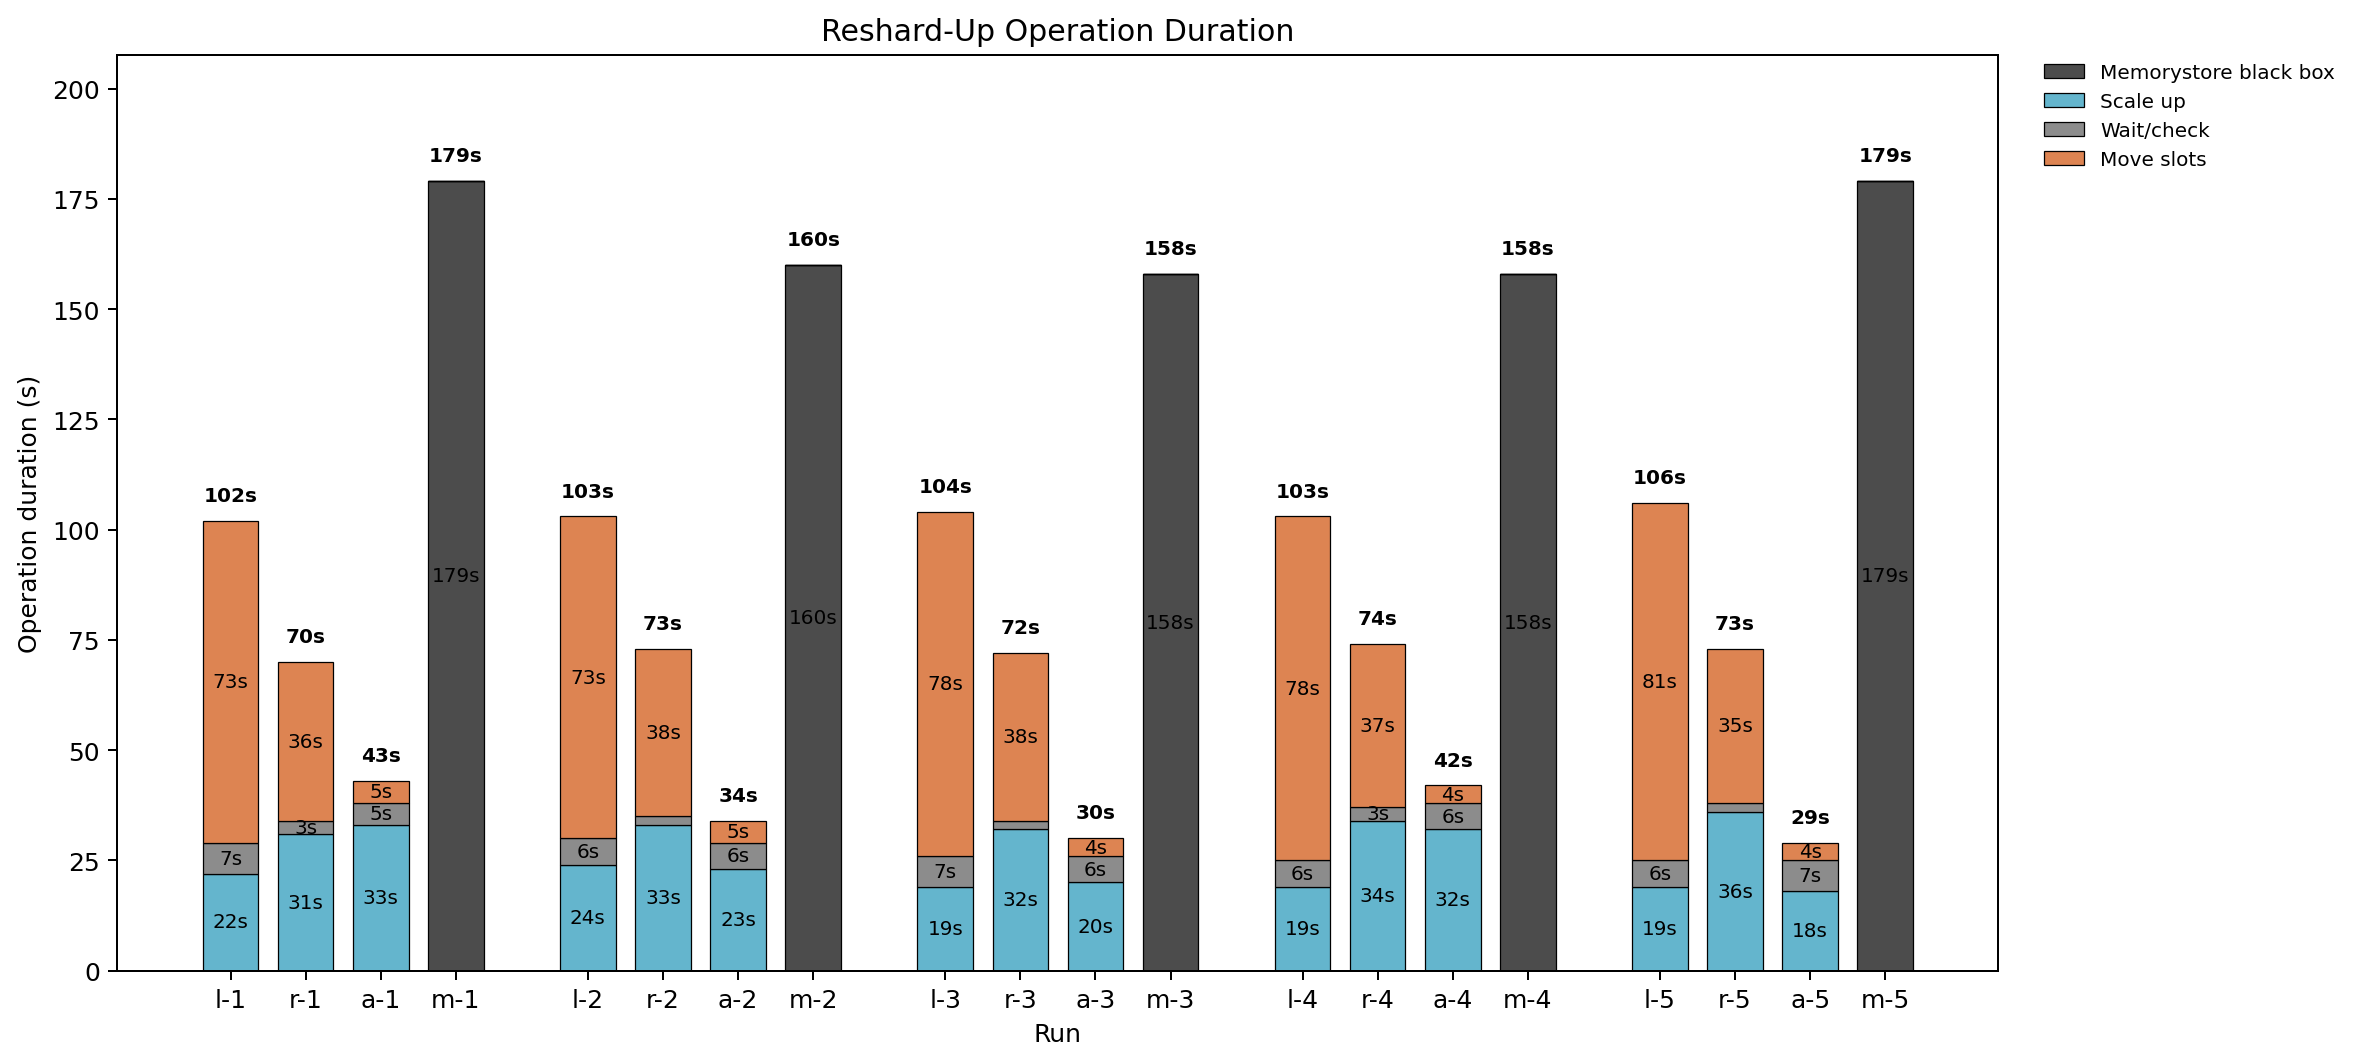
\includegraphics[width=\textwidth]{images/reshard_up_comparison.png}
    \caption{Porównanie czasu skalowania z trzech do czterech shardów dla migracji legacy, migracji atomowej oraz Memorystore.}
    \label{fig:reshard-up-comparison}
\end{figure}

\begin{figure}[!htbp]
    \centering
    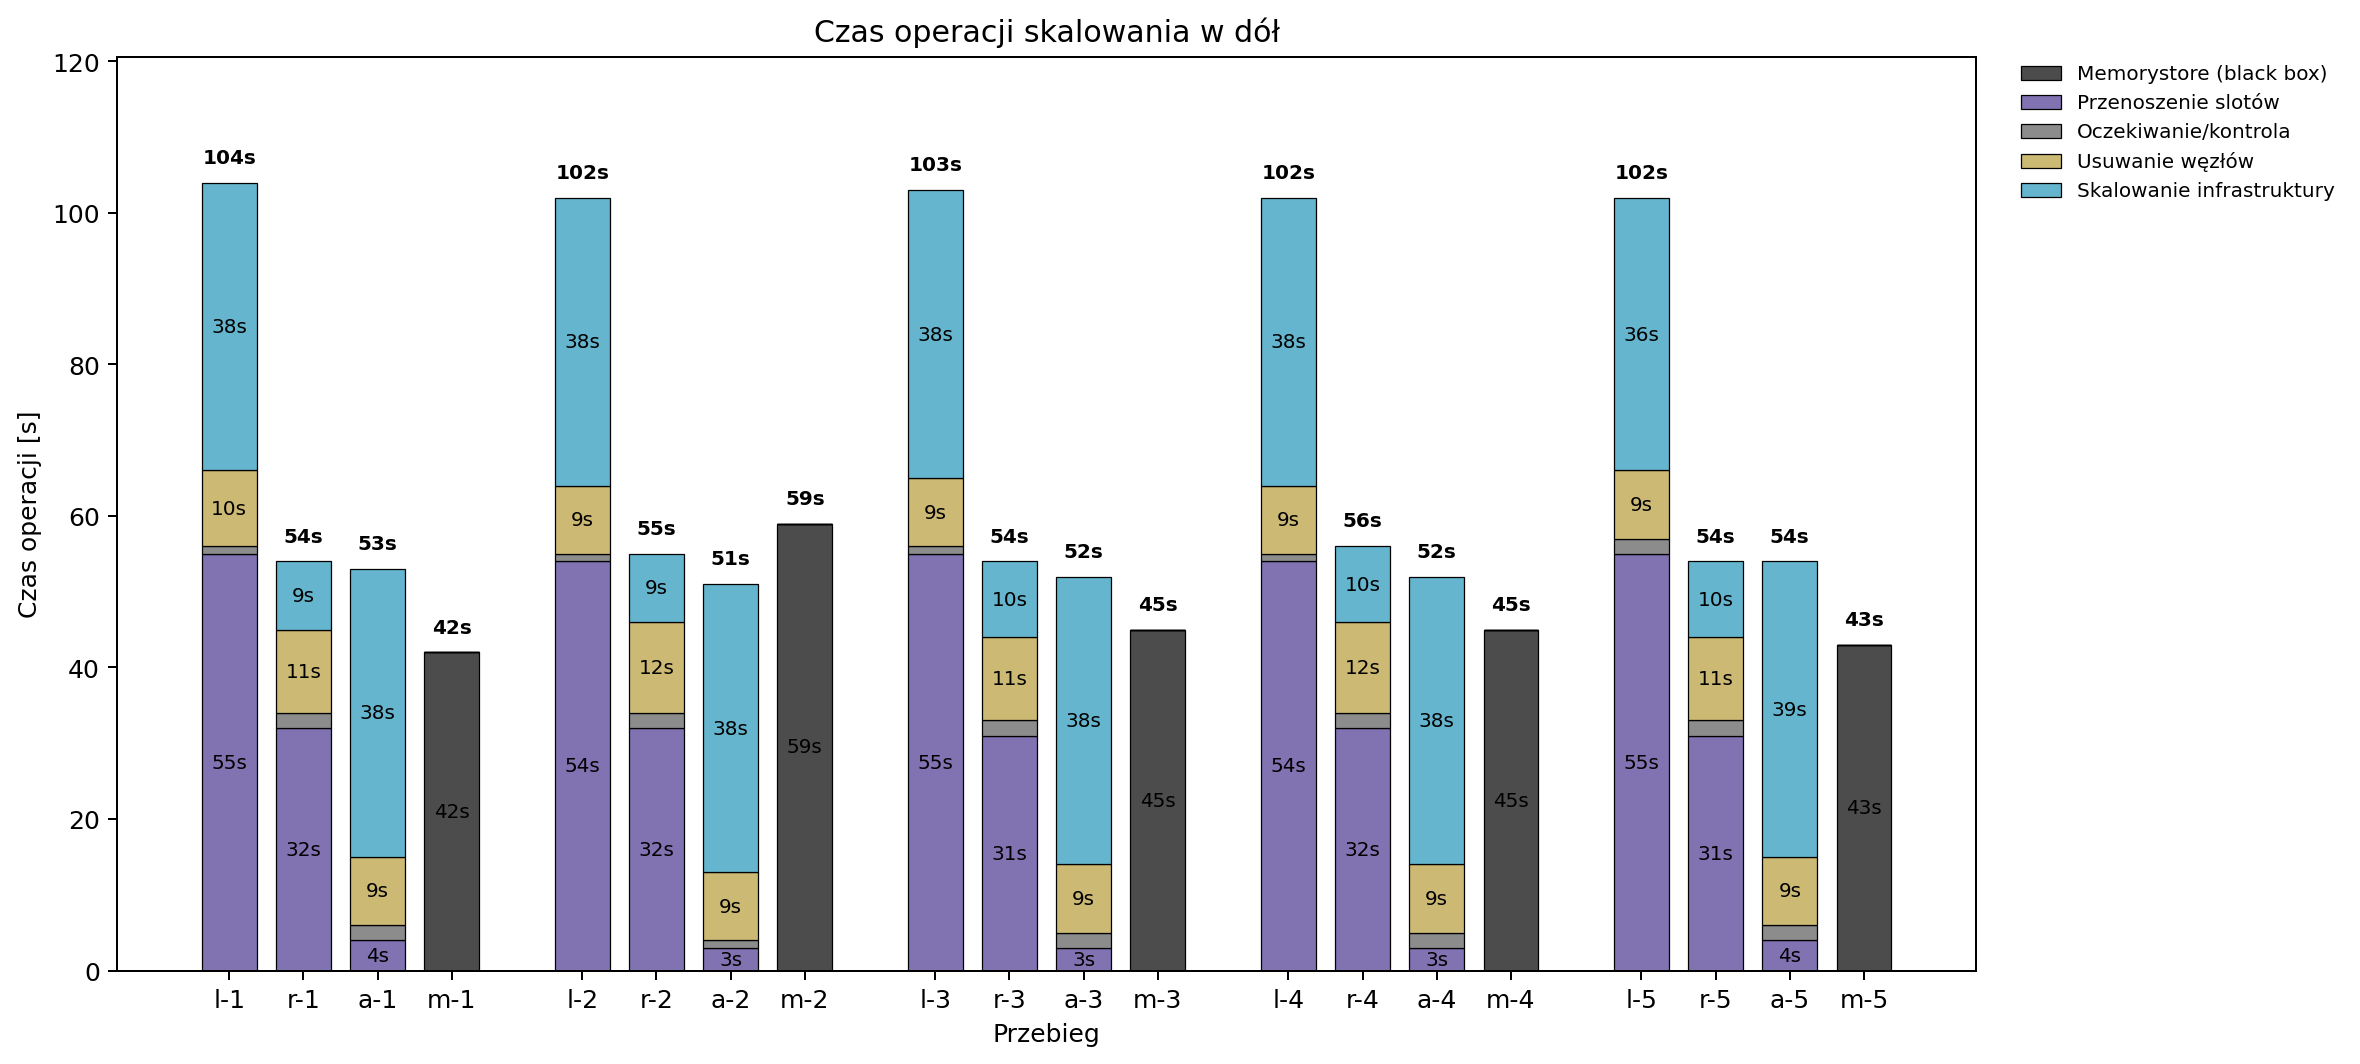
\includegraphics[width=\textwidth]{images/reshard_down_comparison.png}
    \caption{Porównanie czasu skalowania z czterech do trzech shardów dla migracji legacy, migracji atomowej oraz Memorystore.}
    \label{fig:reshard-down-comparison}
\end{figure}

\FloatBarrier

Tabela~\ref{tab:reshard-duration} pokazuje średni czas całej operacji administracyjnej wraz z odchyleniem standardowym. Przyspieszenie zostało policzone względem klasycznej migracji slotów Valkey w tej samej fazie testu.

\begin{table}[htbp]
\centering
\caption{Czas reshardingu i przyspieszenie względem migracji legacy.}
\label{tab:reshard-duration}
\begin{adjustbox}{max width=\textwidth}
\begin{tabular}{lrrrrr}
\toprule
Faza & Legacy [s] & Atomic [s] & Memorystore [s] & Atomic / legacy & Memorystore / legacy \\
\midrule
3 $\rightarrow$ 4 shardy & $103{,}6 \pm 1{,}5$ & $35{,}6 \pm 6{,}6$ & $166{,}8 \pm 11{,}2$ & $2{,}91\times$ & $0{,}62\times$ \\
4 $\rightarrow$ 3 shardy & $144{,}8 \pm 6{,}8$ & $55{,}6 \pm 0{,}5$ & $46{,}8 \pm 6{,}9$ & $2{,}60\times$ & $3{,}09\times$ \\
\bottomrule
\end{tabular}
\end{adjustbox}
\end{table}

\FloatBarrier

Największa różnica między trybem legacy i atomic pojawia się w fazie wykonywanej przez \texttt{valkey-cli --cluster rebalance}. Przy skalowaniu w górę klasyczna migracja zajmowała średnio 76{,}6~s, podczas gdy migracja atomowa 4{,}4~s. Przy skalowaniu w dół różnica była jeszcze bardziej widoczna w części odpowiedzialnej za opróżnienie dodatkowego sharda: 96{,}0~s dla legacy oraz 4{,}0~s dla atomic.

Wynik Memorystore jest asymetryczny. Skalowanie z trzech do czterech shardów trwało średnio 166{,}8~s, czyli dłużej niż oba warianty Valkey self-hosted. Skalowanie z czterech do trzech shardów trwało jednak średnio 46{,}8~s i było szybsze od obu wariantów self-hosted liczonych jako pełna operacja administracyjna.

Wpływ reshardingu na klienta przedstawia tabela~\ref{tab:reshard-latency-throughput}. Wartości percentyli są średnimi z wyników raportowanych przez \texttt{memtier\_benchmark} dla pięciu powtórzeń, natomiast kolumna \textit{ops/sec} zawiera średnią oraz odchylenie standardowe.

\begin{table}[htbp]
\centering
\caption{Przepustowość i percentyle opóźnień podczas reshardingu.}
\label{tab:reshard-latency-throughput}
\begin{adjustbox}{max width=\textwidth}
\begin{tabular}{llrrrrr}
\toprule
Faza & Wariant & Ops/sec & p50 [ms] & p95 [ms] & p99 [ms] & p99.9 [ms] \\
\midrule
3 $\rightarrow$ 4 & Legacy & $105\,999{,}91 \pm 1\,144{,}62$ & 1{,}27 & 6{,}17 & 10{,}97 & 19{,}97 \\
3 $\rightarrow$ 4 & Atomic & $112\,655{,}54 \pm 2\,069{,}61$ & 1{,}28 & 5{,}49 & 10{,}16 & 19{,}53 \\
3 $\rightarrow$ 4 & Memorystore & $141\,327{,}99 \pm 1\,985{,}12$ & 1{,}23 & 2{,}01 & 2{,}95 & 6{,}71 \\
4 $\rightarrow$ 3 & Legacy & $101\,685{,}72 \pm 635{,}51$ & 1{,}62 & 7{,}05 & 11{,}98 & 22{,}07 \\
4 $\rightarrow$ 3 & Atomic & $114\,688{,}15 \pm 2\,664{,}65$ & 1{,}18 & 5{,}24 & 9{,}41 & 18{,}38 \\
4 $\rightarrow$ 3 & Memorystore & $140\,837{,}06 \pm 1\,026{,}09$ & 1{,}47 & 2{,}42 & 3{,}54 & 7{,}45 \\
\bottomrule
\end{tabular}
\end{adjustbox}
\end{table}

\FloatBarrier

Podczas obu faz atomic utrzymał wyższą przepustowość niż legacy oraz niższe opóźnienia w ogonie rozkładu. Dla skalowania w dół p99 spadło z 11{,}98~ms do 9{,}41~ms, a p99.9 z 22{,}07~ms do 18{,}38~ms. Memorystore osiągnął najwyższą przepustowość i najniższe percentyle opóźnień, ale ten wynik należy zestawiać z innym charakterem środowiska: usługa zarządzana działa poza kontrolowanym klastrem Kubernetes i ukrywa część mechanizmów administracyjnych. Z punktu widzenia testu self-hosted najważniejszy wniosek jest taki, że atomowa migracja slotów znacząco skraca okno reshardingu i jednocześnie ogranicza degradację opóźnień względem klasycznej migracji.

\section{Rolling upgrade klastra Valkey}

Celem testu rolling upgrade było sprawdzenie, jak klaster Valkey zachowuje się podczas aktualizacji wersji wykonywanej pod obciążeniem. Procedura testu, parametry \texttt{memtier\_benchmark} oraz sposób działania klienta kontrolnego zostały opisane w podrozdziale~\ref{subsec:rolling_upgrade}. Wyniki dla pięciu powtórzeń przedstawiono w tabeli~\ref{tab:upgrade-results}.

\begin{table}[htbp]
\centering
\caption{Wyniki testu rolling upgrade z perspektywy klienta kontrolnego.}
\label{tab:upgrade-results}
\begin{adjustbox}{max width=\textwidth}
\begin{tabular}{rrrrrrr}
\toprule
Przebieg & Czas [s] & Próby & Błędy & Timeouty & Error rate [\%] & p99 [ms] \\
\midrule
1 & 281 & 1153 & 16 & 11 & 1{,}39 & 111{,}44 \\
2 & 290 & 1202 & 15 & 10 & 1{,}25 & 39{,}99 \\
3 & 268 & 1136 & 15 & 6 & 1{,}32 & 40{,}95 \\
4 & 282 & 1205 & 13 & 6 & 1{,}08 & 35{,}96 \\
5 & 269 & 1136 & 16 & 7 & 1{,}41 & 34{,}65 \\
\midrule
Śr. $\pm$ odch. std. & $278{,}0 \pm 9{,}35$ & $1166{,}4 \pm 34{,}6$ & $15{,}0 \pm 1{,}22$ & $8{,}0 \pm 2{,}35$ & $1{,}29 \pm 0{,}13$ & $52{,}60 \pm 33{,}00$ \\
\bottomrule
\end{tabular}
\end{adjustbox}
\end{table}

\FloatBarrier

Średni czas rolling upgrade wyniósł 278~s. W oknie aktualizacji klient kontrolny zarejestrował średnio 15 błędów na około 1166 prób, co odpowiada 1{,}29\% nieudanych operacji. Najczęściej były to timeouty operacji \texttt{SET}; pojawiały się również odpowiedzi \texttt{CLUSTERDOWN} oraz pojedyncze błędy połączenia. Podczas rozruchu oraz po zakończeniu aktualizacji nie zarejestrowano błędów.

\section{Backup i restore}

Celem testu było porównanie czasu wykonania kopii zapasowej i odtworzenia klastra dla dwóch wariantów: samodzielnie utrzymywanego klastra Valkey w Kubernetes z backupem opartym o snapshoty GCE Persistent Disk oraz zarządzanego klastra Redis w Google Cloud Memorystore z wbudowanym mechanizmem backupu. Procedura testu, fazy operacji oraz sposób weryfikacji integralności zostały opisane w podrozdziale~\ref{subsec:backup_restore}. Dla każdego wariantu wykonano po pięć powtórzeń na zbiorze danych o rozmiarze 10\,240~MB (10\,485\,760 kluczy).

\subsection{Valkey self-hosted --- PVC snapshots}

Tabela~\ref{tab:backup-valkey-phases} przedstawia średni czas poszczególnych faz backupu i odtworzenia wraz z odchyleniem standardowym. Rozbicie na fazy pokazano na rysunku~\ref{fig:valkey-backup-breakdown}.

\begin{table}[htbp]
\centering
\caption{Czas poszczególnych faz backupu i restore dla klastra Valkey (5 powtórzeń, 10~GB danych).}
\label{tab:backup-valkey-phases}
\begin{adjustbox}{max width=\textwidth}
\begin{tabular}{lrr}
\toprule
Faza & Średni czas [s] & Odch. std. [s] \\
\midrule
\multicolumn{3}{l}{\textit{Backup}} \\
\quad BGSAVE & $12{,}2$ & $0{,}84$ \\
\quad Skalowanie StatefulSet do 0 & $33{,}2$ & $0{,}84$ \\
\quad Tworzenie snapshotów dysków & $220{,}2$ & $5{,}63$ \\
\quad \textbf{Łączny czas backupu} & $\mathbf{266{,}0}$ & $\mathbf{5{,}39}$ \\
\midrule
\multicolumn{3}{l}{\textit{Restore}} \\
\quad Tworzenie dysków ze snapshotów & $133{,}0$ & $0{,}00$ \\
\quad Tworzenie PV/PVC & $9{,}8$ & $3{,}70$ \\
\quad Uruchomienie podów & $22{,}0$ & $0{,}71$ \\
\quad Odzyskanie stanu klastra & $3{,}0$ & $2{,}74$ \\
\quad \textbf{Łączny czas restore} & $\mathbf{169{,}8}$ & $\mathbf{5{,}02}$ \\
\midrule
Weryfikacja integralności (10\% próbka) & $256{,}2$ & $10{,}47$ \\
\bottomrule
\end{tabular}
\end{adjustbox}
\end{table}

\begin{figure}[!htbp]
    \centering
    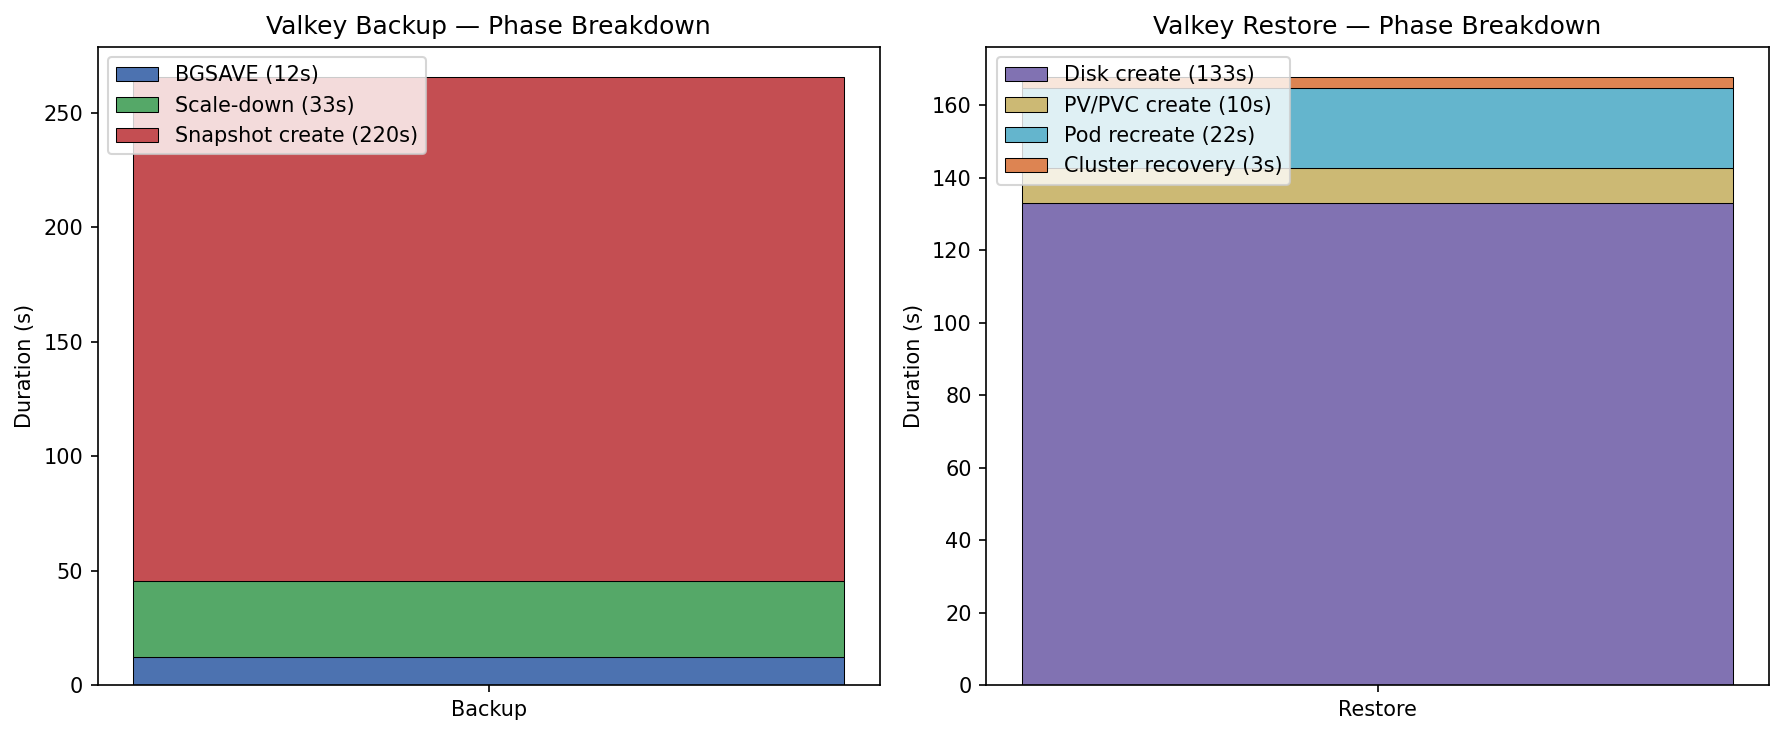
\includegraphics[width=\textwidth]{images/valkey_backup_phase_breakdown.png}
    \caption{Rozbicie czasu backupu i restore klastra Valkey na poszczególne fazy.}
    \label{fig:valkey-backup-breakdown}
\end{figure}

\FloatBarrier

Dominującą fazą backupu jest tworzenie snapshotów dysków GCE (średnio 220{,}2~s, co stanowi 83\% całkowitego czasu backupu). Sam zapis RDB trwał jedynie 12{,}2~s. Po stronie odtworzenia najdłuższą operacją jest tworzenie dysków ze snapshotów (133{,}0~s, 78\% czasu restore). Czas uruchomienia podów i osiągnięcia gotowości klastra wyniósł łącznie 25~s.

Integralność danych została potwierdzona w 4 z 5 przebiegów. W przebiegu numer 4 weryfikator zgłosił 3 błędy na próbce 1\,048\,576 kluczy (0{,}0003\%), przy zerowej liczbie brakujących kluczy. Ponieważ żadne klucze nie zostały utracone, błędy te mogą wynikać z różnicy w momencie wykonania BGSAVE na poszczególnych shardach.

\subsection{Memorystore --- zarządzany backup}

Tabela~\ref{tab:backup-memorystore} przedstawia wyniki dla usługi Memorystore.

\begin{table}[htbp]
\centering
\caption{Czas backupu i restore dla Memorystore (5 powtórzeń, 10~GB danych).}
\label{tab:backup-memorystore}
\begin{adjustbox}{max width=\textwidth}
\begin{tabular}{lrr}
\toprule
Faza & Średni czas [s] & Odch. std. [s] \\
\midrule
Backup (zarządzany) & $49{,}4$ & $8{,}14$ \\
Restore (utworzenie klastra z backupu) & $475{,}4$ & $17{,}90$ \\
Weryfikacja integralności & $470{,}4$ & $8{,}93$ \\
\bottomrule
\end{tabular}
\end{adjustbox}
\end{table}

\FloatBarrier

Backup zarządzany trwał średnio 49{,}4~s, co jest ponad pięciokrotnie szybsze od wariantu self-hosted (266{,}0~s). Wynika to z faktu, że Memorystore nie wymaga zatrzymania klastra ani tworzenia snapshotów wolumenów --- usługa wykonuje kopię wewnętrznie. Natomiast operacja odtworzenia (utworzenie nowego klastra z backupu) trwała średnio 475{,}4~s, czyli prawie trzykrotnie dłużej niż restore w wariancie self-hosted (169{,}8~s). Wynika to z konieczności alokacji i konfiguracji nowej infrastruktury klastra przez dostawcę chmurowego. Integralność danych została potwierdzona we wszystkich pięciu przebiegach.

\subsection{Porównanie wariantów}

Rysunek~\ref{fig:backup-comparison} zestawia czasy backupu i restore obu wariantów. Tabela~\ref{tab:backup-comparison-total} podsumowuje łączny czas operacji.

\begin{figure}[!htbp]
    \centering
    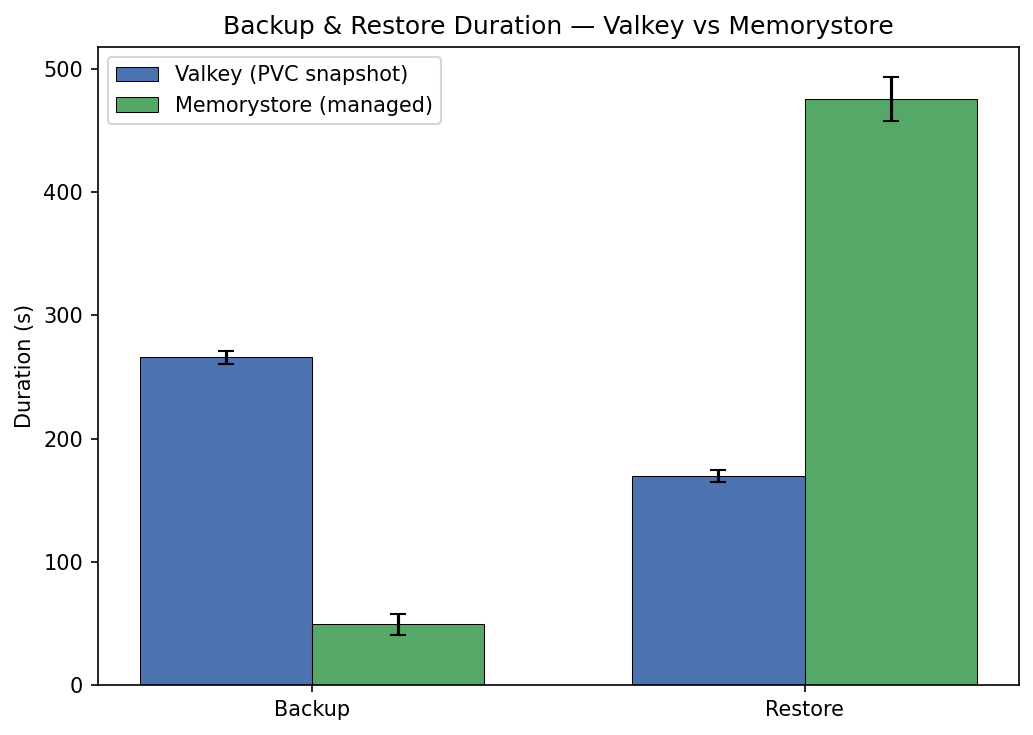
\includegraphics[width=0.85\textwidth]{images/backup_comparison.png}
    \caption{Porównanie czasu backupu i restore między Valkey self-hosted a Memorystore.}
    \label{fig:backup-comparison}
\end{figure}

\begin{table}[htbp]
\centering
\caption{Porównanie łącznego czasu backupu i restore.}
\label{tab:backup-comparison-total}
\begin{adjustbox}{max width=\textwidth}
\begin{tabular}{lrrr}
\toprule
Operacja & Valkey [s] & Memorystore [s] & Stosunek \\
\midrule
Backup & $266{,}0 \pm 5{,}4$ & $49{,}4 \pm 8{,}1$ & $5{,}38\times$ \\
Restore & $169{,}8 \pm 5{,}0$ & $475{,}4 \pm 17{,}9$ & $0{,}36\times$ \\
Łącznie (backup + restore) & $435{,}8$ & $524{,}8$ & $0{,}83\times$ \\
\bottomrule
\end{tabular}
\end{adjustbox}
\end{table}

\FloatBarrier

Warianty prezentują odwrócone proporcje: Memorystore oferuje szybki backup (5{,}4$\times$ krótszy), ale wolny restore (2{,}8$\times$ dłuższy). Łączny czas cyklu backup--restore jest w wariancie self-hosted krótszy o~17\% (435{,}8~s vs 524{,}8~s). Kluczowa różnica operacyjna polega na tym, że backup Valkey wymaga niedostępności klastra na czas skalowania w dół i tworzenia snapshotów (łącznie ${\sim}253$~s), natomiast backup Memorystore nie powoduje przestoju w obsłudze zapytań.

\chapter{Podsumowanie i wnioski z badań}\label{ch:podsumowanie}

\section{Podsumowanie badań}

W ramach pracy przeprowadzono siedem kategorii testów porównawczych obejmujących badania wydajności, resharding, failover mastera, spójność danych podczas partycji sieciowej, odporność na niedobór zasobów (CPU i pamięć), rolling upgrade oraz backup i restore. Każdy test był powtarzany pięciokrotnie ($N = 5$). Wyniki poddano analizie statystycznej z~wykorzystaniem dwustronnego testu Manna-Whitneya~U na poziomie istotności $\alpha = 0{,}05$. W~scenariuszach z~wieloma porównaniami zastosowano korektę Benjaminiego-Hochberga (FDR). Łącznie przeprowadzono 66~testów statystycznych, z~których 49~wykazało istotną różnicę.

\section{Weryfikacja hipotez badawczych}

\textbf{H1} (wydajność): W~15~z~18~konfiguracji wydajnościowych różnica w~przepustowości między Valkey a Redis 7.2 była istotna statystycznie po korekcie FDR ($p_{\mathrm{adj}} < 0{,}05$, $|r| \geq 0{,}84$). Valkey osiągał wyższą przepustowość niż Redis 7.2 przy payloadach 1~KB (wszystkie proporcje operacji, oba limity vCPU) oraz przy payloadzie 1000~KB w~trybie write-only i mieszanym. Trzy konfiguracje z~payloadem 10~KB nie wykazały istotnej różnicy, co wskazuje na nasycenie przepustowości ograniczone przepływnością pamięci lub sieci. Jedyny przypadek, w~którym Redis 7.2 wykazał wyższe nominalne ops/sec (1000~KB read-only, stosunek $0{,}07$), okazał się artefaktem pomiarowym: w~tym profilu Redis obsługiwał ok.\ 93\% chybień (tanie odpowiedzi \texttt{nil}), więc liczba ta nie odzwierciedlała odczytu dużych wartości --- po uwzględnieniu rzeczywistej przepustowości danych (\texttt{KB/sec}) oba systemy obsługiwały duże odczyty praktycznie identycznie (zob.\ rozdz.~\ref{ch:wyniki}). Analogiczna analiza percentyla p99 opóźnień wykazała istotną różnicę w~14~z~18~konfiguracji.

Hipotezę H1 uznaje się za \textit{częściowo potwierdzoną}: Valkey osiąga istotnie wyższą przepustowość w~większości konfiguracji (szczególnie przy payloadach 1~KB i 1000~KB write/mixed), natomiast przy payloadach 10~KB różnice są statystycznie nieistotne (nasycenie przepustowości). Nie zaobserwowano przy tym konfiguracji, w~której Redis 7.2 byłby rzeczywiście szybszy --- jedyny taki przypadek (1000~KB read-only) wynikał z~różnicy w~trafieniach, a~nie z~wydajności silnika.

\textbf{H2} (koszty): Infrastruktura self-hosted kosztuje 699{,}29~USD/mies.\ wobec 804{,}17~USD/mies.\ dla Memorystore w~regionie \texttt{europe-central2} przy cenach on-demand --- self-hosted jest o~13\% tańszy. Nawet po doliczeniu opłaty za zarządzanie klastrem GKE (73~USD/mies.) koszt self-hosted (772{,}29~USD) pozostaje poniżej Memorystore. Jednocześnie warianty self-hosted wymagają 7--11~kroków proceduralnych i 5--12~komend operatora w~scenariuszach upgrade, resharding i backup/restore, wobec 1--6~kroków i 1--5~komend dla Memorystore. Wobec ograniczeń uniemożliwiających przeprowadzenie dedykowanego testu wydajnościowego Memorystore, koszt jednostkowy na 100~tys.\ ops/sec wyznaczono z~przepustowości baseline testu reshardingu (30-sekundowe okno stanu ustalonego przed operacją): wynosi on $\approx$344~USD zarówno dla Valkey, jak i~dla Redis 7.2 (zbliżona przepustowość $\approx$203~tys.\ ops/sec) oraz $\approx$567~USD dla Memorystore ($\approx$142~tys.\ ops/sec). Hipotezę H2 uznaje się za \textit{potwierdzoną}: infrastruktura self-hosted jest tańsza od Memorystore w~badanej konfiguracji, a~w~jedynym zmierzonym profilu osiąga przy tym wyższą przepustowość; wiąże się to jednak z~wyższym nakładem pracy operacyjnej.

\textbf{H3} (failover): Test Manna-Whitneya~U nie wykazał istotnej różnicy w~czasie failoveru między Valkey a Redis 7.2 ($p = 0{,}23$). Oba systemy wykazały zbliżony czas okna błędów ($\approx$18~s), spadek przepustowości ($\approx$35\%) i liczbę błędów połączenia ($\approx$244). Hipotezę H3 uznaje się za \textit{niepotwierdzoną} w~części dotyczącej krótszego czasu failoveru Valkey. Oba warianty zachowują się równoważnie pod względem promocji repliki. Część hipotezy dotycząca porównywalności z~Memorystore nie mogła zostać zweryfikowana eksperymentalnie.

\textbf{H4} (utrzymywalność): Valkey self-hosted wymaga 7~kroków i 5~komend przy rolling upgrade, 7--8~kroków i 5--6~komend przy reshardingu oraz 11~kroków i 12~komend przy backup/restore. Memorystore wymaga odpowiednio 4~kroków/2~komendy (resharding) i 6~kroków/5~komend (backup/restore). Testy wykazały jednocześnie, że atomowa migracja slotów w~Valkey jest istotnie szybsza od wszystkich pozostałych wariantów przy skalowaniu w~górę ($p_{\mathrm{adj}} \leq 0{,}011$), a~czas odtworzenia Valkey jest istotnie krótszy od Redis 7.2 ($p = 0{,}008$) i Memorystore ($p = 0{,}012$). Hipotezę H4 uznaje się za \textit{potwierdzoną}: wariant self-hosted wymaga więcej kroków proceduralnych, ale oferuje krótsze czasy operacji.

\section{Wnioski}

\begin{enumerate}
    \item Valkey stanowi funkcjonalną i wydajnościową alternatywę dla Redis 7.2 w~środowisku Kubernetes. W~większości testowanych konfiguracji oferuje istotnie wyższą przepustowość przy zachowaniu porównywalnej lub niższej latencji.
    \item Oba systemy są nieodróżnialne statystycznie pod względem failoveru i spójności danych podczas partycji sieciowej (brak istotnych różnic przy $N = 5$), co jest spójne ze~wspólnym modelem asynchronicznej replikacji Redis Cluster.
    \item Atomowa migracja slotów (dostępna od Valkey 9.0) istotnie skraca czas reshardingu i~zmniejsza wpływ operacji na opóźnienia klienta.
    \item Valkey lepiej radzi sobie z~presją pamięci (wyższe ops/sec, niższe p99 pod polityką \texttt{allkeys-lru}), natomiast wzorzec degradacji pod stresem CPU jest bardziej złożony i~zależy od liczby dotkniętych masterów.
    \item Memorystore oferuje niższy nakład pracy operacyjnej, ale w~regionie \texttt{europe-central2} jest o~13\% droższy od infrastruktury self-hosted (804~USD vs 699~USD/mies.) przy cenach on-demand. Memorystore ma jednocześnie dłuższe czasy odtworzenia i~reshardingu w~górę. W~jedynym profilu, w~którym udało się zmierzyć przepustowość Memorystore (baseline testu reshardingu), osiągała ona $\approx$142~tys.\ ops/sec wobec $\approx$203~tys.\ ops/sec dla self-hosted, co przekłada się na niższy koszt jednostkowy self-hosted ($\approx$344 wobec $\approx$567~USD na 100~tys.\ ops/sec); różnicę przepustowości częściowo tłumaczy dodatkowy skok sieciowy klienta do usługi zarządzanej.
\end{enumerate}

\section{Rekomendacje praktyczne dla przemysłu}

Na podstawie uzyskanych wyników można sformułować następujące rekomendacje dla zespołów projektujących i~utrzymujących klastry Redis-kompatybilne w~środowiskach produkcyjnych:

\begin{enumerate}
    \item \textbf{Valkey jako zamiennik Redis 7.2.} Dla większości typowych obciążeń (payloady rzędu pojedynczych kilobajtów, proporcje read/write zbliżone do mieszanych) Valkey stanowi bezpieczny zamiennik Redis 7.2 --- oferuje istotnie wyższą przepustowość przy tym samym modelu replikacji oraz nieodróżnialnym statystycznie zachowaniu podczas failoveru i~partycji sieciowej. Migracja nie wymaga zmian po stronie aplikacji klienckiej dzięki zachowaniu zgodności protokołu.
    \item \textbf{Weryfikacja pod kątem konkretnego profilu obciążenia.} Przewaga wydajnościowa nie jest uniwersalna --- przy payloadach 10~KB różnice między systemami okazały się statystycznie nieistotne. Dodatkowo wynik 1000~KB read-only pokazuje, jak łatwo o~błędną interpretację: nominalne ops/sec mogą być zawyżone przez chybienia (\texttt{nil}) przy zbiorze danych większym niż \texttt{maxmemory}. Przed migracją zaleca się przeprowadzenie testu na reprezentatywnym profilu, z~kontrolą współczynnika trafień i~rzeczywistej przepustowości danych (\texttt{KB/sec}), zamiast polegania na samej nominalnej liczbie operacji.
    \item \textbf{Wybór self-hosted vs.\ usługa zarządzana.} Samodzielnie zarządzany klaster w~Kubernetes jest tańszy (o~$\approx$13\% w~koszcie infrastruktury i~$\approx$344 wobec $\approx$567~USD w~koszcie jednostkowym na 100~tys.\ ops/sec w~badanym profilu), ale wymaga wyższego nakładu pracy operacyjnej (7--11~kroków proceduralnych w~scenariuszach utrzymaniowych). Rozwiązanie self-hosted rekomenduje się zespołom dysponującym kompetencjami w~zakresie Kubernetes, dla których koszt i~kontrola nad konfiguracją są priorytetem; Memorystore --- zespołom optymalizującym czas i~nakład operacyjny kosztem wyższej ceny.
    \item \textbf{Atomowa migracja slotów przy reshardingu.} W~klastrach Valkey (od~wersji~9.0) zaleca się włączenie atomowej migracji slotów --- skraca ona czas reshardingu i~istotnie ogranicza wpływ operacji skalowania na opóźnienia po stronie klienta w~porównaniu z~klasycznym mechanizmem.
    \item \textbf{Obciążenia z~intensywną eksmisją.} Dla cache'y działających pod presją pamięci z~polityką \texttt{allkeys-lru} Valkey osiągał wyższą przepustowość i~niższe p99 niż Redis 7.2, co czyni go preferowanym wyborem dla scenariuszy z~częstą eksmisją kluczy.
    \item \textbf{Współlokowanie klienta z~klastrem.} Niższa przepustowość obserwowana wobec Memorystore wynikała częściowo z~dodatkowego skoku sieciowego klienta do usługi zarządzanej. W~projektach wrażliwych na opóźnienia zaleca się umieszczanie aplikacji klienckich możliwie blisko węzłów klastra (ta sama strefa/sieć), niezależnie od wybranego wariantu wdrożenia.
\end{enumerate}

\section{Weryfikacja osiągnięcia celu pracy}

Celem pracy była analiza porównawcza klastra Valkey w~Kubernetes z~rozwiązaniami opartymi o~Redis. Cel został osiągnięty: przeprowadzono pomiary wydajności, niezawodności i utrzymywalności w~siedmiu scenariuszach testowych, potwierdzono lub odrzucono cztery hipotezy badawcze z~wykorzystaniem testów statystycznych, a~wyniki przedstawiono w~formie ilościowej z~podaniem p-wartości i~wielkości efektu.
\chapter{Zakończenie}\label{ch:zakonczenie}

Celem pracy była kompleksowa analiza porównawcza samodzielnie zarządzanego klastra Valkey uruchomionego w~Kubernetes z~klastrem Redis~7.2 oraz z~usługą zarządzaną Google Cloud Memorystore for Redis, prowadzona pod kątem wydajności, opóźnień, odporności na awarie, kosztów oraz nakładu pracy operacyjnej. Postawiony problem badawczy --- czy Valkey może stanowić praktyczną, wydajną i~ekonomicznie uzasadnioną alternatywę dla Redis~7.2 i~rozwiązania zarządzanego --- doczekał się odpowiedzi opartej na pomiarach w~siedmiu kategoriach testów, powtarzanych pięciokrotnie i~poddanych analizie statystycznej z~korektą na wielokrotne porównania.

Zgromadzony materiał pozwala stwierdzić, że Valkey jest dojrzałą i~funkcjonalnie zgodną alternatywą dla Redis~7.2. W~większości profili obciążenia osiąga istotnie wyższą przepustowość, przy payloadach pośrednich (10~KB) różnice są statystycznie nieistotne, a~jedyny przypadek pozornej przewagi Redis (odczyt dużych wartości) okazał się artefaktem współczynnika trafień, a~nie cechą silnika. Pod względem zachowania podczas awarii mastera oraz spójności danych w~trakcie partycji sieciowej oba systemy są statystycznie nieodróżnialne, co jest spójne ze~wspólnym modelem asynchronicznej replikacji. Z~kolei atomowa migracja slotów dostępna w~nowszych wersjach Valkey istotnie skraca czas reshardingu i~ogranicza jego wpływ na klienta. Z~perspektywy ekonomicznej infrastruktura self-hosted okazała się tańsza od usługi zarządzanej, kosztem wyższego nakładu pracy operacyjnej.

Rezultaty pracy mają zarówno charakter poznawczy, jak i~użytkowy. W~warstwie poznawczej pokazano, że deklarowana zgodność interfejsu między Valkey a~Redis przekłada się na zgodność obserwowanego zachowania w~scenariuszach produkcyjnych, oraz że pozornie spektakularne różnice w~surowych metrykach mogą wynikać z~konfiguracji i~sposobu pomiaru, a~nie z~architektury silnika. W~warstwie użytkowej praca dostarcza zestawu rekomendacji oraz powtarzalnej metodyki i~narzędzi benchmarkowych, które organizacja stojąca przed decyzją migracyjną po zmianie licencji Redis może wykorzystać do oceny własnego obciążenia.

Przeprowadzone badania mają jednak ograniczenia, które wyznaczają granice wniosków. Badania wydajności prowadzono w~środowisku lokalnym (minikube) ze~względu na ograniczony dostęp do zasobów chmurowych, co zawyża wartości bezwzględne przepustowości i~utrudnia bezpośrednie przeniesienie ich do środowiska produkcyjnego. Liczba powtórzeń ($N=5$) jest wystarczająca do testów nieparametrycznych, ale ogranicza moc wykrywania drobnych różnic. Dedykowanego, pełnego testu wydajnościowego usługi Memorystore nie udało się zrealizować z~powodu ograniczeń zasobowych --- jej przepustowość oszacowano jedynie z~jednego profilu zarejestrowanego w~teście reshardingu, z~dodatkowym narzutem skoku sieciowego klienta. Porównanie samodzielnie zarządzanych klastrów i~usługi zarządzanej nie odbywa się też w~identycznym środowisku, a~różnice między użytymi chartami Helm (valkey-helm oraz Bitnami) wprowadzają asymetrie konfiguracji, których nie da się w~pełni wyeliminować.

Naturalnym kierunkiem dalszych prac jest powtórzenie testów wydajnościowych w~jednorodnym środowisku chmurowym o~większej skali, z~pełną macierzą profili obciążenia również dla Memorystore, oraz zwiększenie liczby powtórzeń w~celu uzyskania węższych przedziałów ufności. Wartościowe byłoby również zbadanie wpływu trwałości danych (AOF, snapshoty), szyfrowania TLS oraz dłuższych, bardziej złożonych scenariuszy chaos engineering na wnioski dotyczące niezawodności. Osobnym wątkiem jest domknięcie analizy zaobserwowanej asymetrii eksmisji przez porównanie efektywnych konfiguracji silników na działających instancjach, a~także automatyzacja operacji utrzymaniowych za pomocą operatorów Kubernetes, co mogłoby zmniejszyć przewagę usług zarządzanych w~obszarze nakładu pracy operacyjnej.


% BIBLIOGRAFIA - https://www.overleaf.com/learn/latex/Bibliography_management_with_bibtex
\resetformatting
\cleardoublepage
\phantomsection
\pagestyle{bibliographyStyle}
\addcontentsline{toc}{chapter}{Bibliografia}
\bibliographystyle{plabbrv-fixed}
\bibliography{bibliography}

% SPIS RYSUNKOW
\cleardoublepage
\phantomsection
\pagestyle{custom}
\pagestyle{ListofFiguresStyle}
\addcontentsline{toc}{chapter}{Spis rysunków}
\listoffigures

% SPIS TABEL
\clearpage
\phantomsection
\pagestyle{ListofTablesStyle}
\addcontentsline{toc}{chapter}{Spis tabel}
\listoftables

% SPIS ALGORYTMOW
\clearpage
\phantomsection
\pagestyle{ListofAlgorithmsStyle}
\addcontentsline{toc}{chapter}{Spis algorytmów}
\listofalgorithms

% SPIS KODOW ZRODLOWYCH
\clearpage
\phantomsection
\pagestyle{ListofListingsStyle}
\addcontentsline{toc}{chapter}{Spis kodów źródłowych}
\lstlistoflistings

\end{document}